%%%%%%%%%%%%%%%%%%%%%%%%%%%%%%%%%%%%%%%%%
% Masters/Doctoral Thesis 
% LaTeX Template
% Version 1.43 (17/5/14)
%
% This template has been downloaded from:
% http://www.LaTeXTemplates.com
%
% Original authors:
% Steven Gunn 
% http://users.ecs.soton.ac.uk/srg/softwaretools/document/templates/
% and
% Sunil Patel
% http://www.sunilpatel.co.uk/thesis-template/
%
% License:
% CC BY-NC-SA 3.0 (http://creativecommons.org/licenses/by-nc-sa/3.0/)
%
% Note:
% Make sure to edit document variables in the Thesis.cls file
%
%%%%%%%%%%%%%%%%%%%%%%%%%%%%%%%%%%%%%%%%%

%----------------------------------------------------------------------------------------
%	PACKAGES AND OTHER DOCUMENT CONFIGURATIONS
%----------------------------------------------------------------------------------------

\documentclass[11pt,oneside]{Thesis} % The default font size and one-sided printing (no margin offsets)

\graphicspath{{Pictures/}} % Specifies the directory where pictures are stored

\usepackage{lscape}
\usepackage{pgfgantt}
\usepackage{listings}
\usepackage[square, numbers, comma, sort&compress]{natbib}
\usepackage{hyperref}
\usepackage{mathtools}
\usepackage{lscape}
\usepackage{pdflscape}
\usepackage{longtable}
\usepackage{xr}
\usepackage{textcomp}
\usepackage{caption}
\usepackage[english]{babel}
\usepackage{amssymb,amsmath,amsxtra,amsthm,amsfonts}
\usepackage{tocloft}

 % Use the natbib reference package - read up on this to edit the reference style; if you want text (e.g. Smith et al., 2012) for the in-text references (instead of numbers), remove 'numbers' 
\hypersetup{urlcolor=blue, colorlinks=true} % Colors hyperlinks in blue - change to black if annoying
\title{\ttitle} % Defines the thesis title - don't touch this

\begin{document}

\frontmatter % Use roman page numbering style (i, ii, iii, iv...) for the pre-content pages

\setstretch{1.3} % Line spacing of 1.3

% Define the page headers using the FancyHdr package and set up for one-sided printing
\fancyhead{} % Clears all page headers and footers
\rhead{\thepage} % Sets the right side header to show the page number
\lhead{} % Clears the left side page header

\pagestyle{fancy} % Finally, use the "fancy" page style to implement the FancyHdr headers

\newcommand{\HRule}{\rule{\linewidth}{0.5mm}} % New command to make the lines in the title page

% PDF meta-data
\hypersetup{pdftitle={\ttitle}}
\hypersetup{pdfsubject=\subjectname}
\hypersetup{pdfauthor=\authornames}
\hypersetup{pdfkeywords=\keywordnames}

%----------------------------------------------------------------------------------------
%	TITLE PAGE
%----------------------------------------------------------------------------------------

\begin{titlepage}
\begin{center}

\textsc{\LARGE \univname}\\[1.5cm] % University name
\textsc{\Large PAWI}\\[0.5cm] % Thesis type

\HRule \\[0.4cm] % Horizontal line
{\huge \bfseries \ttitle}\\[0.4cm] % Thesis title
\HRule \\[1.5cm] % Horizontal line
 
\begin{minipage}{0.4\textwidth}
\begin{flushleft} \large
\emph{Author:}\\
{\authornames} % Author name - remove the \href bracket to remove the link
\end{flushleft}
\end{minipage}
\begin{minipage}{0.4\textwidth}
\begin{flushright} \large
\emph{Supervisors:} \\
{\supname} \linebreak \linebreak  % Supervisor name - remove the \href bracket to remove the link  
\emph{Examiners:} \\
{\examname}\\
\end{flushright}
\end{minipage}\\[3cm]
 
 
{\large \today}\\[4cm] % Date
%\includegraphics{Logo} % University/department logo - uncomment to place it
 
\vfill
\end{center}

\end{titlepage}

%----------------------------------------------------------------------------------------
%	DECLARATION PAGE
%	Your institution may give you a different text to place here
%----------------------------------------------------------------------------------------

\Declaration{

\addtocontents{toc}{\vspace{1em}} % Add a gap in the Contents, for aesthetics

I, \authornames, declare that this thesis titled, '\ttitle' and the work presented in it are my own. I confirm that:

\begin{itemize} 
\item[\tiny{$\blacksquare$}] This work was done wholly or mainly while in candidature for a research degree at this University.
\item[\tiny{$\blacksquare$}] Where any part of this thesis has previously been submitted for a degree or any other qualification at this University or any other institution, this has been clearly stated.
\item[\tiny{$\blacksquare$}] Where I have consulted the published work of others, this is always clearly attributed.
\item[\tiny{$\blacksquare$}] Where I have quoted from the work of others, the source is always given. With the exception of such quotations, this thesis is entirely my own work.
\item[\tiny{$\blacksquare$}] I have acknowledged all main sources of help.
\item[\tiny{$\blacksquare$}] Where the thesis is based on work done by myself jointly with others, I have made clear exactly what was done by others and what I have contributed myself.\\
\end{itemize}
 
Signed:\\
\rule[1em]{25em}{0.5pt} % This prints a line for the signature
 
Date:\\
\rule[1em]{25em}{0.5pt} % This prints a line to write the date
}

\clearpage % Start a new page


%----------------------------------------------------------------------------------------
%	ABSTRACT PAGE
%----------------------------------------------------------------------------------------

\addtotoc{Abstract} % Add the "Abstract" page entry to the Contents

\abstract{\addtocontents{toc}{\vspace{1em}} % Add a gap in the Contents, for aesthetics

TODOs:
\begin{itemize}
\item abstract
\item check for forgotten cites
\item ask lengi why this stupid list of table/figure is not working

\end{itemize}
}

\clearpage % Start a new page

%----------------------------------------------------------------------------------------
%	ACKNOWLEDGEMENTS
%----------------------------------------------------------------------------------------

% \setstretch{1.3} % Reset the line-spacing to 1.3 for body text (if it has changed)

% \acknowledgements{\addtocontents{toc}{\vspace{1em}} % Add a gap in the Contents, for aesthetics

%  \ldots
% }
% \clearpage % Start a new page

%----------------------------------------------------------------------------------------
%	LIST OF CONTENTS/FIGURES/TABLES PAGES
%----------------------------------------------------------------------------------------

\pagestyle{fancy} % The page style headers have been "empty" all this time, now use the "fancy" headers as defined before to bring them back

\lhead{\emph{Contents}} % Set the left side page header to "Contents"
\tableofcontents % Write out the Table of Contents


\pagebreak
\lhead{\emph{List of Figures}} % Set the left side page header to "List of Figures"
\listoffigures % Write out the List of Figures
\thispagestyle{empty}

\pagebreak
\lhead{\emph{List of Tables}} % Set the left side page header to "List of Tables"
\listoftables % Write out the List of Tables
\thispagestyle{empty}

%----------------------------------------------------------------------------------------
%	ABBREVIATIONS
%----------------------------------------------------------------------------------------

\clearpage % Start a new page

\setstretch{1.5} % Set the line spacing to 1.5, this makes the following tables easier to read

\lhead{\emph{Abbreviations}} % Set the left side page header to "Abbreviations"
\listofsymbols{ll} % Include a list of Abbreviations (a table of two columns)
{
\textbf{PAWI} & \textbf{P} \textbf{A} \textbf{W} \textbf{I}\\
\textbf{HTML} & \textbf{H}yper \textbf{T}ext \textbf{M}arkup \textbf{L}anguage \\
\textbf{BTE} & \textbf{B}ody \textbf{T}ext \textbf{E}xtraction \\
\textbf{DOM} & \textbf{D}ocument \textbf{O}bject \textbf{M}odel \\
\textbf{TP} & \textbf{T}rue \textbf{P}ositive \\
\textbf{TN} & \textbf{T}rue \textbf{N}egative \\
\textbf{FP} & \textbf{F}alse \textbf{P}ositive \\
\textbf{FN} & \textbf{F}alse \textbf{N}egative \\
\textbf{TV} & \textbf{T}ele\textbf{V}ision \\
\textbf{IDE} & \textbf{I}ntegrated \textbf{D}evelopment \textbf{E}nvironment \\
\textbf{CI}  & \textbf{C}ontinuous \textbf{I}ntegration \\
\textbf{RSS}  & \textbf{R}ich \textbf{S}ide \textbf{S}ummary \\
\textbf{API}  & \textbf{A}pplication \textbf{P}rogramming \textbf{I}nterface \\
\textbf{JDK}  & \textbf{J}ava \textbf{D}evelopment \textbf{K}it \\
\textbf{f x}  & \textbf{f}eature x\\
\textbf{MS x}  & \textbf{M}ile\textbf{S}tone x\\
\textbf{tc x} & \textbf{t}est \textbf{c}ase x \\
\textbf{TPR} & \textbf{T}rue \textbf{P}ositive \textbf{R}ate \\ 
\textbf{FPR} & \textbf{F}alse \textbf{P}ositive \textbf{R}ate \\ 
\textbf{CSV} & \textbf{C}omma \textbf{S}separated \textbf{V}alues \\
\textbf{DSL} & \textbf{D}omain \textbf{S}pecific \textbf{L}anguage \\
\textbf{XML} & E\textbf{X}tensible \textbf{M}arkup \textbf{L}anguage\\
}



%----------------------------------------------------------------------------------------
%	DEDICATION
%----------------------------------------------------------------------------------------

\setstretch{1.3} % Return the line spacing back to 1.3

\pagestyle{empty} % Page style needs to be empty for this page

\dedicatory{For/Dedicated to/To my\ldots} % Dedication text

\addtocontents{toc}{\vspace{2em}} % Add a gap in the Contents, for aesthetics

%----------------------------------------------------------------------------------------
%	THESIS CONTENT - CHAPTERS
%----------------------------------------------------------------------------------------

\mainmatter % Begin numeric (1,2,3...) page numbering

\pagestyle{fancy} % Return the page headers back to the "fancy" style

% Include the chapters of the thesis as separate files from the Chapters folder
% Uncomment the lines as you write the chapters

% Chapter Template

\chapter{Problem statement} % Main chapter title

\label{Problem statement} % Change X to a consecutive number; for referencing this chapter elsewhere, use \ref{ChapterX}

\lhead{\emph{Problem statement}} % Change X to a consecutive number; this is for the header on each page - perhaps a shortened title

%----------------------------------------------------------------------------------------
%	SECTION 1
%----------------------------------------------------------------------------------------

This chapter describes the problem statement, as well as the topical environment in which the project takes place.


\section{Introduction}

This project is done on behalf of the company Layzapp. Layzapp is specialized in second-screen solutions. It is currently working on a mobile application which brings relevant data to a second screen during a TV show. The Internet is crawled to find relevant information about a certain topic. The outcome of this search is a certain number of web pages. The content of these web pages is made usable by removing irrelevant data, such as navigation elements, advertisement and login pages. Removing the HTML content is not a very hard task. But after this first process of removal there is still much irrelevant content left, for instance descriptions of further articles or advertisements. Removing this part is much more complicated. 

\section{Task}

As described in the introduction, irrelevant content, which is also called boilerplate, needs to be removed from a web page. There are already several algorithms which fulfill this task. To compare the performance of the known algorithms and contrast them to possible new algorithms, a test environment is required. The test environment needs to classify the quality of a text extraction performed by the different algorithms. For this purpose, each algorithm is fed with a certain amount of HTML content. The outcome is then inspected for its quality. 

 \section{Text extraction and algorithms}

 This chapter is a description of the text extraction subject and the known algorithms.

 \subsection{Text extraction}

 Text extraction or content extraction of web pages is a widely discussed field in research. There are several approaches to this field. The two main approaches are page segmentation via visual and DOM features and boilerplate removal. The main drawback of visual page segmentation is that at some point the web page needs to be rendered and processed as image. This task is very time-consuming and many resources are necessary to fulfill it. This project focuses on algorithms which work with boilerplate removal.
 The basic idea of boilerplate removal was first introduced with the BTE (Body Text Extraction) algorithm. The assumptions are the relevant part of the HTML content is usually a contiguous stretch, the density of HTML tags is lower in it that in boilerplate content. Hence, by breaking up the HTML page in single sections and counting the HTML tags, there is an area where the number of HTML tags do not increase. It is quite simple to define an objective function. One can expect that this is the article text. Unfortunately, BTE's performance is very limited, but it is still used to compare different extraction algorithms to each other. The two algorithms Boilerpipe and Justext improve the performance of BTE.

 \subsection{Boilerpipe}

 The Boilerpipe algorithm is based on the concept described in Kohlschütter's paper "Boilerplate Detection using Shallow Text Features". It uses a variate of HTML tags  to divide the HTML document into blocks. Each block is classified according to its shallow text features and to the classification of the  previous and the next blocks. Some examples for shallow text features are average word length, average sentence length or the absolute number of words. The features are described more closely in the paper.

 \subsection{Justext}

Justext uses similar features as Boilerplate but inspects the data for the presence of stop words as well. Some examples for stop words are "a", "and", "but", "how", "or", and "what". An article contains more stop words than boilerplate. Based on this information, a better classification can be achieved.

\subsection{Classification}

The main task of the application is to somehow classify the performance of the algorithms. The performance can be defined as how much of relevant text is classified as relevant and how much is classified as boilerplate. In information retrieval, these performances can be described in a confusion matrix.

\begin{table}[h]
\begin{tabular}{|p{4cm} |p{5.5cm} |p{5.5cm} |}\hline
          								& \textbf{Classified as content} 	& \textbf{Classified as boilerplate} 	\\ \hline
\textbf{Actual content} 				& True positive (TP)				& False negative(FN)					\\ \hline
\textbf{Actual boilerplate} 			& False positive (FP)       		& True negative (TN)				 	\\ \hline
\end{tabular}
\end{table}

\begin{itemize}
\item True positive is the amount of text which is relevant content and classified as content by the algorithm
\item False positive is the amount of text which is relevant content but classified as boilerplate by the algorithm 
\item True negative is the amount of text which is boilerplate and is classified as boilerplate by the algorithm
\item False negative is the amount of text which is boilerplate but is classified as content by the algorithm
\end{itemize}

These values are the basis for calculating  both the recall (also known as sensitivity) which is the fraction of relevant text that is retrieved and the precision which is the fraction of retrieved text that is relevant. These values, their dependencies and some more values are described more closely in the software requirement specification (\ref{subsec:Evaluation of classification}).

\section{Conclusion}

An application is needed which can be fed with HTML documents. These documents are then processed by text extraction algorithms. The outcome is then compared with the relevant content and classification values are calculated. Based on these values the performance of the algorithms can be compared. Possible strengths and weaknesses can be determined in this comparison.


i% Chapter Template

\chapter{Solution development} % Main chapter title

\label{Solution development} % Change X to a consecutive number; for referencing this chapter elsewhere, use \ref{ChapterX}

\lhead{\emph{Solution development}} % Change X to a consecutive number; this is for the header on each page - perhaps a shortened title

%----------------------------------------------------------------------------------------
%	SECTION 1
%----------------------------------------------------------------------------------------

This chapter describes the approach developing the application. It does not cover each and every detail of the project. Only the key problems are discussed. However, all the topics are described more closely in the related project documents in the appendices.

\section{Approach}

\subsection{Planning}

The planning of this project was a very straight forward task. Since it is a small one man project and the start and end dates were clearly defined.  However I am working part time for Layzapp and this project was not my only task during the period of time and the project needed to be coordinated with other tasks. My solution was to work about one to two weeks for this project and switch to other tasks for the next one to two weeks. Switching between multiple projects within one week seemed not very effective because one always needs some hours to get back into a topic. \linebreak
A project plan was done for the whole time line. Five milestones and their delivery objects were defined. As we were working with scrum a milestone was defined as sprint and the delivery objects were divided into stories on the start of each sprint. Since it was a one man team no weekly scrum meetings were done. There was a sprint meeting at the end of each sprint and the delivery objects were presented to the supervisors and the tasks for the next sprint were redefined. During the project, the tool toggl (\ref{sec:Time tracking}) was used as a time tracker and task manager. The whole planning as well as the time tracking can be found in appendix \ref{Planning}.

\subsection{Programming}

As a first step the development environment was set up. The used tools were

\begin{itemize}
\item IDE: Eclipse
\item Version control: Git hosted on GitHub
\item CI server: Travis CI
\item Build tool: Gradle
\end{itemize}

These tools are described in more detail in appendix \ref{architecture:developmentView}. 

As soon as the whole continuous integration process was working, a data model and a first approach of the software architecture was developed. This first approach was implemented so that the basic functionality of the application was working. With this working version the data model and the software architecture could be tested and approved.

The next step was to eliminate the biggest risk, the integration of the two algorithms JusText and Boilerpipe into the application. Prototypes for the algorithms were programmed. Integrating the Boilerpipe algorithm \cite{algo:boilerpipe}  was easy since it is implemented in Java and could be used without the need of any modification. Integrating the JusText algorithm \cite{algo:justext} was a more difficult because it is implemented in Python. The final solution was to call the python application with system calls from the java application and read the output text file generated by the python program.

The second big risk was the approach comparing the text of the actual content with the outcome of the algorithms and find the classification values (TP, TN, FP, FN). The different approaches are described for the following example.


The text file with the expected test results contains following text.


\texttt{I am an interesting text. My content is about advertisement in modern times.}

The extracted text file by an algorithm contains following text.

\texttt{I am an interesting text. And i am an advertisement for socks. }

The first approach was counting each word in the content file and checking if the same amount of words are available in the extracted text file. In doing so words could occur in different places in a text but could still be classified as correct. This is presented in the example. The word 'advertisement' in the content file is part of the actual content. In the extracted text file, the sentence 'My content is about advertisement in modern times.' is not found but there is still a text passage classified as content where the word 'advertisement' occurs. As a result, the word advertisement would be classified as correct (True positive) with this first approach because it is counted once in each text. So this approach could not be used.
In a second approach, the comparison was done by not only comparing a single word but as well as the word before and after the word of interest. 
For the example above, for each word, a group of three words is built and this group is then compared with the second text. The word 'advertisement' would be defined as the word group 'about advertisement in' and the second text is searched for this pattern. Since there is no such group, the word advertisement would be classified wrong (False positive) which would be the correct classification. With this approach the results were already a lot better. But there were still situations where this approach was not working. Instead of implementing an elaborated text comparison algorithm we decided to fall back on existing solutions. Text file comparison tools like diff \cite{wiki:diff} or meld \cite{wiki:meld} are doing exactly the task we were looking for. We decided to use the open source implementation merge-diff-patch \cite{google:diffMatchPatch} developed by google.  The outcome of the comparison performed by diff-match-patch are all the words of the input text grouped in 'EQUAL', 'DELETE' and 'INSERT' which can be easy transferred into the needed values True Positive ('EQUAL'), False Positive ('INSERT'), True Negative ('DELETE') and False Negative (remaining words). 


The next task after handling these risks was to integrate the prototypes into the main application. The remaining programming tasks were then refactoring the first approach and testing the application. The final software architecture is described in the abbreviation under Appendix \ref{architecture}. The test concept is described under Appendix \ref{Test plan}. 

The final programming task would have been the implementation of a new text extraction algorithm. On the MS4 meeting ( Appendix \ref{ms4report}), we decided not to implement an additional text extraction algorithm because we needed to investigate the problems of the existing algorithms first so that we have a better idea what we need to improve for our own algorithm. So instead of focusing on a new approach, we decided to focus improving the test framework. 
The improvement focus on the following two problems. It was not possible to filter test cases of interest from the whole test set and it was not possible to get specific information about one specific test case.

\subsection{Filtering results}
The first needed improvement was the possibility of filtering all the test cases for a certain criterion. To do so, a new configuration item was defined which could be added to the configuration file before starting the test run. The filter function is explained with the following example.

If one wants to have all test cases were JusText had a good rating for precision and Boilerplate did not, the following lines could be added to the configuration file.

\begin{lstlisting}
filter:justext:precision:min:0.8;
filter:boilerpipe:precision:max:0.2;
\end{lstlisting} 

Every test case which has precision value below 80\% for JusText and a precision value above 20\% for Boilerpipe was now removed from the results. The resulting test cases were all test cases where JusText performed quite well and Boilerpipe did not. These test cases can then be investigated more closely.
With this new function it became much easier to investigate certain test cases in more detail.

\subsection{Evaluation based on blocks}

The second needed improvement was the possibility to evaluate a single test instead of all tests.
The most information about a single test such as Precision, Recall and the extracted text by the algorithms was already available. The more challenging part was to get the classification based on the blocks generated by the algorithms. Neither Justext nor Boilerpipe have an API call to get the output results including the classification information for the individual blocks. Which means that the two algorithms needed to be modified.

\subsubsection{Modifications of JusText}
\label{subsec:Modification JusText}

Even with no prior knowledge at the programming language python, the task was easier then expected. The algorithm is working with blocks during the whole process and prints the blocks classified as content. All we needed to do is to print the classification values at the beginning of each block and parse the output string accordingly with the main application.
This is an example of the printed string after my modification. \linebreak

\begin{lstlisting}
<p class="bad" cfclass="bad" heading="0" word_count="3" link_density="1" 
stopword_count="1" stopword_density="0"> Kites with Antennas
\end{lstlisting}

First, all the classification data like 'link density' and 'stop word count' was printed followd by the text of the actual block. Which is 'Kites with Antennas' in the example above. This string can then be parsed by the test framework for further use.


\subsubsection{Modifications to Boilerpipe}

Adapting the Boilerpipe algorithm on the other hand was not as easy as expected. Boilerpipe does merge the single blocks while the algorithm is being carried out and the classification information for some blocks is lost due to this approach. My solution was to change the algorithm so that each block is backed up before it is merged with other blocks with all its available classification information. The problem with this approach is that some blocks are re-classified differently at a later point in time and the backed up data is not correct anymore. Bigger changes of the algorithm would be needed to solve this problem but this would go beyond the scope of this project. Nevertheless, the initial classification can be extracted and this already helps to find possible problems and as well compare it with the results from other algorithms.


\section{Results}


\subsection{Statistical data}

With the test framework it was finally possible to produce the classification data for the  algorithms using an HTML source file and a content file as input data. Doing this with a few test files, it is not possible to produce a concrete quality criterion for an algorithm. A bigger test data set was needed. In the context of a text extraction competition called CleanEval \cite{CleanEval:online}, a large large data set was gathered for their needs. This data set meets the demands of this project in every respect. We decided to use this data set instead of gathering our own data set at the MS1 meeting (\ref{reports:ms1report}). 
The following table shows the overall results when extracting the CeanEval test files with JusText and Boilerpipe and process the results with the test framework.


\begin{tabular}{| p{2.2cm} | p{2.2cm} | p{2.2cm} | p{2.2cm} | p{2.2cm} | p{2.2cm} |}
    \hline
    \textbf{Algorithm}      & \textbf{Precision}  & \textbf{Recall}  & \textbf{Fallout}  & \textbf{F-Measure}  &\textbf{Accuracy} \\ \hline
    JusText     & 95.29 \%       &  91.99 \%  & 35.03 \% & 91.37 \% & 85.11 \%   \\ \hline
    Boilerpipe & 95.15 \%       &  74.38 \%  & 49.31 \% & 79.56 \% &  68.17 \% \\ \hline

\end{tabular}

The meaning of the single result types is described in Appendix section \ref{subsec:Evaluation of classification}.



\subsection{Analysis}

This test data was not only used in this but also in other papers, which broach the issue of text extraction. The paper 'More Effective Boilerplate Removal—the GoldMiner Algorithm' \cite{paper:goldminer} used the same test data to compare their Goldminer algorithm to JusText and Boilerpipe. The results from this paper were used to verify my approach is heading into the right direction or if the outcome is completely wrong. 
The results from the paper testing the different algorithms with the gold standard  are shown in table \ref{table:resultsGoldminer}.

\begin{table}[!ht]
\begin{tabular}{| p{3cm} | p{3cm} | p{3cm} | }
    \hline
    \textbf{Algorithm}      & \textbf{Precision}  & \textbf{Recall} 				\\ \hline
    JusText     & 95.29 \%       &  91.99 \%		\\ \hline
    Boilerpipe & 95.15 \%       &  74.38 \%		\\ \hline
\end{tabular}
\caption[asdfasdf]{The results for the CleanEval test set from the Goldminer paper}
\label{table:resultsGoldminer}
\end{table}

The results from my test framework are shown in table \ref{table:resultsComparison} 

\begin{table}[!ht]
\begin{tabular}{| p{3cm} | p{3cm} | p{3cm} | }
    \hline
    \textbf{Algorithm}      & \textbf{Precision}  & \textbf{Recall} 				\\ \hline
    JusText     & 95.86 \%       &  87.27 \%		\\ \hline
    Boilerpipe & 91.14 \%       &  70.60 \%		\\ \hline
\end{tabular}
\caption{The results for the CleanEval test set from the test framework}
\label{table:resultsComparison}
\end{table}


The results are not exaclty the same but they are close. The difference could be explained by several points. First, there is no guarantee that the results from the Goldminer paper are correct. Second, most of the common approaches comparing these text extraction algorithms were done in comparing the correct classified HTML blocks and not the single words like I did it in this project. This can change the results significantly. Following example should clarify this statement.

Suppose we have an HTML document with ten blocks which have a certain amount of words and are classified by an algorithm as defined in table \ref{blockWordExample}.

\begin{table}[!ht]
\begin{tabular}{| p{2cm} | p{3cm} | p{3cm} | }
    \hline
    \textbf{Block No.}      & \textbf{Word count}  & \textbf{Classification} 				\\ \hline
    1     & 10      	&  True Positive	\\ \hline
    2     & 100     	&  True Positive	\\ \hline
    3     & 50       	&  True positive	\\ \hline
    4     & 30       	&  True Positive	\\ \hline
    5     & 1       	&  False Positive	\\ \hline
    6     & 1000      	&  False Positive	\\ \hline
    7     & 20      	&  False Positive	\\ \hline
    8     & 300       	&  False Positive	\\ \hline
    9     & 200       	&  False Negative	\\ \hline
    10    & 50        	&  False Negative	\\ \hline
\end{tabular}
\caption{Example Blocks vs. Words}
\label{blockWordExample}
\end{table}

The formulas for calculating precision and recall are described in the appendix section \ref{subsec:Evaluation of classification}.
The calculated values for precision and recall from table \ref{blockWordExample} is shown in table \ref{ResultsBlockWordExample}

\begin{table}[!ht]
\begin{tabular}{| p{3cm} | p{5cm} | p{5cm} | }
    \hline
    \ \textbf{Algorithm}  & \textbf{Calculation based on blocks}  & \textbf{Calculation based on words} 				\\ \hline
    Precision     & 50 \%    	&  12.57 \%	\\ \hline
    Recall & 66.67 \%    	&  25.68 \%	\\ \hline
\end{tabular}
\caption{Results example Blocks vs. Words}
\label{ResultsBlockWordExample}
\end{table}

We can see that the difference between the two approaches is quite significant because a large block which is classified wrongs is not weighted as high as if the values are calculated based on blocks instead of words. 
Comparing algorithms based on words seems to be the better approach since the results are more accurate. Furthermore, each algorithm can define the size of a block by itself and the two algorithms do not have to produce the same amount of blocks. Comparing different numbers of blocks does not produce very accurate results either.

\subsection{Detailed analysis}
\label{subsec:Detailed Analysis}

Beside getting these statistical results and comparing the general performance of text extraction algorithms, it is possible to investigate single test cases more closely. To do so, a single line with the test case name needs to be added to the configuration file.

\begin{lstlisting}
inspect:testOfInterest;
\end{lstlisting}

Now the test case 'testOfInterest' is inspected more closely and an extra output file is generated when a test run is performed. Appendix \ref{example:resultsSingleTest} shows an example such a result file.

In the first part, the statistical values are printed followed by the expected content text. Then the results of the tested algorithms are printed, first as continuous text followed by the results formatted as blocks with the according block classification.
The following example shows a single block classified by the algorithms.


\textbf{Boilerpipe}
\begin{lstlisting}
[link_density: 1.0; classification: BOILEPLATE; word_count: 3; stop_Word_Count: 
NOT_DEFINED; text_Density: 3.0; context_Free_classification: NOT_DEFINED; ]
Kites with Antennas
\end{lstlisting}


\textbf{JusText}
\begin{lstlisting}
[link_density: 1.0; classification: BOILEPLATE; word_count: 3; stop_Word_Count: 1; 
text_Density: NOT_DEFINED; context_Free_classification: CFC_BAD; ] 
Kites with Antennas
\end{lstlisting}

The classification values which can be extracted from the algorithms are:

\begin{itemize}
\item Link density,
\item Classification,
\item Word count,
\item Stop word count (only JusText),
\item Text density (Only Boilerpipe),
\item Context free classification (Only justext).
\end{itemize}

Having these values for a certain block already helps evaluating how the algorithms work and why a specific block is classified correct or wrong. Some classification values are only used by one algorithm. These values are marked as 'NOT\_DEFINED' in the output file for the according algorithm.

% Chapter Template

\chapter{Discussion and Outlook} % Main chapter title

\label{Discussion and Outlook} % Change X to a consecutive number; for referencing this chapter elsewhere, use \ref{ChapterX}

\lhead{\emph{Discussion and Outlook}} % Change X to a consecutive number; this is for the header on each page - perhaps a shortened title

%----------------------------------------------------------------------------------------
%	SECTION 1
%----------------------------------------------------------------------------------------

\section {Conclusion}

With the test framework it is now possible to compare text extraction algorithms against each other and get a general information about the performance. We can now rate the performance of the two algorithms JusText and Boilerpipe and with the implemented software architecture it is easy to integrate and test additional algorithms as well. We can not only compare algorithms with each other but as well investigate the single algorithms and their output more closely for specific test cases. This helps to find problems and strengths of existing algorithms and may help to improve them or implement our own algorithm. Based on the results, we can say that JusText performs better context extraction than Boilerpipe.
The missing requirement is the implementation of a new algorithm but with dropping this requirement it was possible to implement the additional functions for investigating the existing algorithms more closely, which will help to improve the existing ones as well as developing a possible new approach in the future.

\section{Lessons learned}

\subsection{Planning}

We did underestimate the effort needed for the documentation. Especially putting together all the single documents and writing the main part took more time then we expected. There are a lot of little things which we did not took in consideration during the planning phase but which need to be done at some point.

\subsection{Programming}
\begin{itemize}
\item It is very important to test software early and often. Most of the critical components were tested right from the beginning. However, if not, a time loss was almost expected for sure because bugs sneaked into the code and needed to be taken care of.

\item I used the programming language Python the first time for this project. Even, only small adjustments on the JusText project needed to be done, a basic knowledge about Python is now present as well as a solution, how to interact with Python from a Java application.

\item I had very basic knowledge about text processing and text extraction. Working with the topic for this project extended my knowledge quite a bit.


\end{itemize}

\section{Further work}

With the test framework we have now the tool to examine text extraction algorithms very close. The next steps will be an exact evaluation of the weaknesses from the algorithms so we can improve them or we can implement our own approach, which handles these problems better. The test framework can then be used at any point during the development phase to check the performance of the algorithm very easy and compare it with the existing ones.  



%----------------------------------------------------------------------------------------
%	THESIS CONTENT - APPENDICES
%----------------------------------------------------------------------------------------

\addtocontents{toc}{\vspace{2em}} % Add a gap in the Contents, for aesthetics

%\appendix % Cue to tell LaTeX that the following 'chapters' are Appendices
% Include the appendices of the thesis as separate files from the Appendices folder
% Uncomment the lines as you write the Appendices

\clearpage
\appendix
\cleardoublepage
\addcontentsline{toc}{chapter}{Appendices}
\addtocontents{toc}{\protect\setcounter{tocdepth}{0}}
\pagenumbering{arabic}
%\blinddocument

% Chapter Template



\chapter{Planning} % Main chapter title

\label{Planning} % Change X to a consecutive number; for referencing this chapter elsewhere, use \ref{ChapterX}

\lhead{Planning \emph{}} % Change X to a consecutive number; this is for the header on each page - perhaps a shortened title

%----------------------------------------------------------------------------------------
%	SECTION 1
%----------------------------------------------------------------------------------------


\section{Planning concept}

So as to plan the project, a combination of the two well known planning frameworks scrum and RUP are used.\\
For a first rough planning, the assignment is split into working packages and assigned to milestones. Delivery objects are defined for each milestone.\\
This plan is then assigned to the given time table of about 12 weeks. The project effort is defined as 180 hours. This results in about 15 hours work load per week.

A more detailed planning is done for the incoming milestone / sprint. The predefined working packages are split into smaller packages. For the first draft, only the first milestone is split into smaller packages. The later milestones are going to be defined in more detail as soon as all needed information is available. 

The effort needed for the documentation is not listed separately. All the tasks already contain additional time for updating the documentation.

The milestones dates are not finally defined, which means that the meeting dates can vary by up to some days.

\section{Milestones overview}

	\begin{tabular}{ | p{3cm} | p{2cm} | p{2cm} | p{2cm} | p{2cm} | p{2cm} |}
	\hline
	\textbf{Name} & \textbf{Shortcut} & \textbf{Weeks} & \textbf{Estimated hours} & \textbf{Hours  \mbox{total}} & \textbf{Closing date} \\ \hline
	Milestone one & m1 & 2.5 & 39 & 39 & 01.10.2014 \\
	Milestone two & m2 & 3 & 45 & 84 & 22.10.2014 \\
	Milestone three & m3 & 2 & 30 & 114 & 05.11.2014 \\
	Milestone four & m4 & 2 & 30 & 144 & 19.11.2014 \\
	Milestone five & m5 & 2.5 & 38 & 182 & 08.12.2014 \\
	\hline
	\end{tabular}


\section{Delivery objects}

    \begin{tabular}{ | p{2.5cm} | p{2.5cm} | p{9cm} |}
    \hline
    \textbf{Milestone} & \textbf{Delivery date} & \textbf{Delivery objects}\\ \hline
    Milestone one & 01.10.2014 &
        \begin{itemize}
        \item System specification
        \item Sketch software architecture
        \item Short presentation CI environment
        \item Draft risk evaluation
        \end{itemize}\\
    \hline
        Milestone two & 22.10.2014 &
        \begin{itemize}
        \item Elaborated software architecture
        \item Tested code of test framework (tbd: which components)
        \item Interface definition for justext/boilerplate components
        \item HTML test data
        \end{itemize}\\
    \hline
        Milestone three & 05.11.2014 &
        \begin{itemize}
        \item Working test environment with both justext and boilerplate components integrated
        \end{itemize}\\
    \hline
        Milestone four & 19.11.2014 &
        \begin{itemize}
        \item Evaluation environment for output data of test framework
        \item First approach to new algorithm
        \end{itemize}\\
    \hline
        Milestone five & 08.12.2014 &
        \begin{itemize}
        \item Implementation of new algorithm
        \item Final documentation
        \item Final presentation
        \end{itemize}\\
    \hline
    \end{tabular}


\section{Milestone one - m1}

\begin{itemize}
\item Closing date date: 1.10.2014
\item Available time: ca. 39h
\end{itemize}

    \begin{tabular}{ | p{10cm} | p{2cm} | p{2cm} |}
    \hline
    \textbf{Story} & \textbf{Shortcut}& \textbf{Estimated time} \\ \hline
    Planning & s1 &4h \\
    Research HTML / Algorithms & s2 & 8h \\
    System specification & s3 & 12h \\
    Risk evaluation & s4 & 3h\\
    Draft software architecture & s5 & 8h \\ 
    Configuration CI environment & s6 & 4h \\ \hline
    Total & & 39h\\
    \hline
    \end{tabular}

\subsection {Stories m1}

    \begin{tabular}{ | p{4cm} | p{10cm} |}
    \hline
    \textbf{Title} & Planning\\ \hline
    \textbf{Id} & s0\\ \hline
    \textbf{Estimated time} & 4h \\ \hline
    \textbf{Description} &  As a project owner, you need to have a time schedule so that you can see when you will achieve which results. The PAWI project is split into several working packages which are then split into single stories. The working packages are assignment to milestones and for each milestone, delivery objects are defined. This can be a document, a piece of test or production code or some other kind of work.\\
    \hline
    \end{tabular} \\\\

    \begin{tabular}{ | p{4cm} | p{10cm} |}
    \hline
    \textbf{Title} & Research HTML / Algorithms\\ \hline
    \textbf{Id} & s1\\ \hline
    \textbf{Estimated time} & 8h \\ \hline
    \textbf{Description} & My knowledge of HTML and content extraction algorithms is still limited. In order to find out what challenges I will face and which aspects I will have to take into consideration for performing the first tasks, a short research on these topics is needed.\\
    \hline
    \end{tabular} \\\\


    \begin{tabular}{ | p{4cm} | p{10cm} |}
    \hline
    \textbf{Title} & System specification\\ \hline
    \textbf{Id} & s2\\ \hline
    \textbf{Estimated time} & 12h \\ \hline
    \textbf{Description} & The PAWI project is defined through a short project description. This description does not cover all necessary information to both plan and perform this project. The key features, interfaces and delivered objects have to be defined more closely. The system specification should cover all these requirements.\\
    \hline
    \end{tabular} \\\\


    \begin{tabular}{ | p{4cm} | p{10cm} |}
    \hline
    \textbf{Title} & Draft software architecture\\ \hline
    \textbf{Id} & s3\\ \hline
    \textbf{Estimated time} & 8h \\ \hline
    \textbf{Description} & A first rough software architecture should be made as soon as possible, so that any misunderstandings between tutors and student can be uncovered. Moreover, it is much easier to plan the further steps when the software is split into several parts.\\
    \hline
    \end{tabular} \\\\


    \begin{tabular}{ | p{4cm} | p{10cm} |}
    \hline
    \textbf{Title} & Risk evaluation\\ \hline
    \textbf{Id} & s4\\ \hline
    \textbf{Estimated time} & 8h \\ \hline
    \textbf{Description} & Potential risks should be uncovered with the knowledge that was gathered by defining the specification and the software architecture. What is more, further actions can be defined to minimize the above mentioned risks.\\
    \hline
    \end{tabular}
    

    \begin{tabular}{ | p{4cm} | p{10cm} |}
    \hline
    \textbf{Title} & Configuration CI environment\\ \hline
    \textbf{Id} & s5\\ \hline
    \textbf{Estimated time} & 4h \\ \hline
    \textbf{Description} & To deliver high quality software a continuous integration environment is required. Following tools should be evaluated and configured for further use:
    \begin{itemize}
        \item Version control (git)
        \item Project build automation tool (gradle)
        \item continuous integration service (Travis CI)
    \end{itemize}
    \\
    \hline
    \end{tabular}


\section{Milestone two - m2}

\begin{itemize}
\item Closing date date: 22.10.2014
\item Available time: ca. 45h
\end{itemize}

    \begin{tabular}{ | p{10cm} | p{2cm} | p{2cm} |}
    \hline
    \textbf{Story} & \textbf{Shortcut}& \textbf{Estimated time} \\ \hline
    Implementation test framework & s6 & 20h \\
    Prototype Integration of justext/boilerpipe & s7 & 17h \\
    Collection of test data & s8 & 8h \\ \hline
    Total &  & 45h\\
    \hline
    \end{tabular}


\subsection {Stories m2}


    \begin{tabular}{ | p{4cm} | p{10cm} |}
    \hline
    \textbf{Title} & Implementation Testframework \\ \hline
    \textbf{Id} & s6\\ \hline
    \textbf{Estimated time} & 20h \\ \hline
    \textbf{Description} & Implementation of a first part of the test framework. This story will be divided into smaller stories as soon as the software architecture and the system specification is reviewed.\\ 
    \hline
    \end{tabular} \\\\


    \begin{tabular}{ | p{4cm} | p{10cm} |}
    \hline
    \textbf{Title} & Prototype Integration of justext/boilerpipe\\ \hline
    \textbf{Id} & s7\\ \hline
    \textbf{Estimated time} & 4h \\ \hline
    \textbf{Description} &  Implementation of a small prototype which uses the existing implementation of justext and boilerpipe. A final interface for both components needs to be defined for further use.
    This story will be divided into smaller stories as soon as the software architecture and the system specification is reviewed.\\ 
    \hline
    \end{tabular} \\\\

    \begin{tabular}{ | p{4cm} | p{10cm} |}
    \hline
    \textbf{Title} & Collection of test data\\ \hline
    \textbf{Id} & s8\\ \hline
    \textbf{Estimated time} & 8h \\ \hline
    \textbf{Description} &  To evaluate the functionality of the text extraction algorithms, a certain amount of test data is needed. This test data contains HTML files of several web pages. The HTML code is categorized into content and boilerplate.\\ 
    \hline
    \end{tabular} \\\\




\section{Milestone three - m3}

\begin{itemize}
\item Closing date date: 5.11.2014
\item Available time: ca. 30
\end{itemize}

    \begin{tabular}{ | p{10cm} | p{2cm} | p{2cm} |}
    \hline
    \textbf{Story} & \textbf{Shortcut}& \textbf{Estimated time} \\ \hline
    Implementation test framework & s9 & 20h \\
    Final integration of justext / boilerplate & s10 & 10h \\ \hline
    Total &  & 30h\\
    \hline
    \end{tabular}

\subsection {Stories m3}

    \begin{tabular}{ | p{4cm} | p{10cm} |}
    \hline
    \textbf{Title} & Implementation test framework \\ \hline
    \textbf{Id} & s9\\ \hline
    \textbf{Estimated time} & 20h \\ \hline
    \textbf{Description} & Final implementation of the test framework. 
    This story will be divided into smaller stories as soon as the software architecture and the system specification is reviewed.\\ 
    \hline
    \end{tabular} \\\\


    \begin{tabular}{ | p{4cm} | p{10cm} |}
    \hline
    \textbf{Title} & Prototype Integration of justext/boilerpipe\\ \hline
    \textbf{Id} & s10\\ \hline
    \textbf{Estimated time} & 4h \\ \hline
    \textbf{Description} &  Complete integration of the justext and boilerplate algorithms into the test framework. 
    This story will be divided into smaller stories as soon as the software architecture and the system specification is reviewed.\\ 
    \hline
    \end{tabular} \\\\





\section{Milestone four - m4}

\begin{itemize}
\item Closing date date: 19.11.2014
\item Available time: ca. 30h
\end{itemize}

    \begin{tabular}{ | p{10cm} | p{2cm} | p{2cm} |}
    \hline
    \textbf{Story} & \textbf{Shortcut}& \textbf{Estimated time} \\ \hline
    Evaluation environment for results & s11 &20h \\
    Research on new algorithm & s12 &10h \\ \hline
    Total &  & 30h\\

    \hline
    \end{tabular}

\subsection {Stories m4}

    \begin{tabular}{ | p{4cm} | p{10cm} |}
    \hline
    \textbf{Title} & Evaluation environment of results\\ \hline
    \textbf{Id} & s11\\ \hline
    \textbf{Estimated time} & 20h \\ \hline
    \textbf{Description} &  The test framework will produce a lot of output data, which has to be reviewed using an evaluation environment. This should process this data and present the results in a descriptive way.
    This story will be divided into smaller stories as soon as the software architecture and the system specification is reviewed.\\ 
    \hline
    \end{tabular} \\\\

        \begin{tabular}{ | p{4cm} | p{10cm} |}
    \hline
    \textbf{Title} & Research on new algorithm\\ \hline
    \textbf{Id} & s12\\ \hline
    \textbf{Estimated time} & 20h \\ \hline
    \textbf{Description} &  A first research on the new algorithm should be performed. After this research it should be possible to decide if this solution is possible and if an implementation with the remaining time resources is realistic.
    This story will be divided into smaller stories as soon as the software architecture and the system specification is reviewed.\\ 
    \hline
    \end{tabular} \\\\


\section{Milestone five - m5}

\begin{itemize}
\item Closing date date: 8.12.2014
\item Available time: ca. 38h
\end{itemize}

    \begin{tabular}{ | p{10cm} | p{2cm} | p{2cm} |}
    \hline
    \textbf{Story} & \textbf{Shortcut}& \textbf{Estimated time} \\ \hline
    Implementation of new algorithm & s13 & 19h \\
    Complete documentation & s14 & 15h \\
    Prepare final presentation & s15 & 4h \\ \hline
    Total &  & 38h\\
    \hline
    \end{tabular}

\subsection {Stories m5}

    \begin{tabular}{ | p{4cm} | p{10cm} |}
    \hline
    \textbf{Title} & Implementation of new algorithm\\ \hline
    \textbf{Id} & s13\\ \hline
    \textbf{Estimated time} & 19h \\ \hline
    \textbf{Description} &  Implementation of the new algorithm and analysis of the test results with the existing evaluation environment. \\ 
    \hline
    \end{tabular} \\\\


    \begin{tabular}{ | p{4cm} | p{10cm} |}
    \hline
    \textbf{Title} & Complete documentation\\ \hline
    \textbf{Id} & s14\\ \hline
    \textbf{Estimated time} & 15h \\ \hline
    \textbf{Description} &  Complete and review all chapters of the documentation.  \\ 
    \hline
    \end{tabular} \\\\

    \begin{tabular}{ | p{4cm} | p{10cm} |}
    \hline
    \textbf{Title} & Prepare final presentation\\ \hline
    \textbf{Id} & s15\\ \hline
    \textbf{Estimated time} & 4h \\ \hline
    \textbf{Description} &  Prepare the final presentation and the final printed / digital version of the thesis.  \\ 
    \hline
    \end{tabular} \\\\











% Chapter Template

\chapter{Risk analysis} % Main chapter title

\label{ChapterX} % Change X to a consecutive number; for referencing this chapter elsewhere, use \ref{ChapterX}

\lhead{\emph{Risk analysis}} % Change X to a consecutive number; this is for the header on each page - perhaps a shortened title

%----------------------------------------------------------------------------------------
%	SECTION 1
%----------------------------------------------------------------------------------------

\section{Risks}

This document evaluates and weights all possible risks and defines actions to minimize them as good as possible.
blublub

\subsection{Unclear requirements}

Requirements are somehow vague at the beginning of each project and if they are not well defined as soon as possible, they stay vague trough out the whole project and this can lead to a disaster. 

\subsection{New technologies}

The new technologies which are present in this project are:

 \begin{itemize}
    \item Gradle
    \item Travis CI
    \item Python
\end{itemize}

Each of them brings his own risk.

\subsection{Interface Boilerpipe}

The Boilerplate algorithm needs to be integrated into the text extraction framework. Every interface of an external component is a possible risk factor.

\subsection{Interface Justext}


The Justext algorithm needs to be integrated into the text extraction framework. Every interface of an external component is a possible risk factor.


\subsection{Implementation RSS algorithm}

The development and implementation of a new algorithm is predestined to generate risks.

\section{Risk analysis}

\begin{table}[h]
\begin{tabular}{|l|c|c|c|}
\hline
\textbf{Risk} & \textbf{Impact} & \textbf{Probability of occurrence} & \textbf{Risk factor} \\ \hline
Unclear requirements & 2 & 4 & 8\\ \hline
New technologies & 3 & 3 & 9 \\ \hline
Interface Boilerpipe & 5 & 1 & 5\\ \hline
Interface Justext & 5 & 5 & 20 \\ \hline
Implementation RSS algorithm & 1 & 5 & 5\\ \hline
\end{tabular}
\end{table}

\section{Consequences}



\subsection{Unclear requirements}

As I am working with the client each and every day, it is very easy prevent missunderstanding with asking the client at once. Even though misunderstandings can occur between student and expert. To prevent this, it is necessary to have a document to define the requirements as soon and as exact as possible. This well be done in the form of the system requirement specification in the first mile stone. Possible ambiguities can be clarified at the first mile stone meeting.

\subsection{New technologies}

It is important to do prototyping with new technologies in the first phase of the project to eliminate these risks as soon as possible.

Gralde and Travic CI are needed in the first mile stone to set up the programming environment. So if there is any problem it will occur in a very early stage of the project and a possible solution can be found.

The risks about python are related to the chapter \ref{subsec:Interface Justext}.

\subsection{Interface Boilerpipe}

This risk is rated much lower than the Justext interface becaus it's implementation is in Java and it provides a Java API. Never then less a prototype should be done as soon as possible to prevent any nasty surprises with the interface.

\subsection{Interface Justext}
\label{subsec:Interface Justext}

This point is classified as the biggest risk of all. This is because the implementation is in Python and it is not clarified yet how it will be integrated into the text extraction framework. An analysis of possible solution with prototypes needs to be done as soon as possible.


\subsection{Implementation RSS algorithm}

This risk has a very high probability of occurrence because it is very likely that a development and an implementation of a new algorithm is going to cause problems. There is no real solution to that risk. But because of this requirement is nice to have, the impact on the outcome of the project is very low. Further more Patrik Lengacher, the tutor of this project, is very experienced in this subject area and will be able to help out if any problems occur. 
% Chapter Template

\chapter{Software Requirement Specification} % Main chapter title

\label{ChapterX} % Change X to a consecutive number; for referencing this chapter elsewhere, use \ref{ChapterX}

\lhead{ \emph{Software Requirement Specification}} % Change X to a consecutive number; this is for the header on each page - perhaps a shortened title

%----------------------------------------------------------------------------------------
%	SECTION 1
%----------------------------------------------------------------------------------------

\section{Version}

\begin{tabular}{| p{1.5cm} | p{2cm} | p{9cm} | p{1.5cm} |}
	\hline
	Version & Date 		& Change & Author \\ \hline
	0.1 	& 20.09.2014 	& Setup document  										& JR \\ \hline
	0.2 	& 28.09.2014		& Add features										& JR \\ \hline
	0.3 	& 30.09.2014		& Change features, grammar, layout					& JR \\ \hline
	0.4 	& 02.10.2014		& Add overview of application/evaluation			& JR \\ \hline
	0.5 	& 04.10.2014		& Corrections evaluation 							& JR \\ \hline
	1.0 	& 05.10.2014		& Grammar, layout 									& JR \\ \hline

\end{tabular}

\section{Introduction}



\subsection{Purpose}

The software requirement specification is providing all needed information to develop the context extraction framework and define all delivery objects. All interfaces to external components, input and output data, deployment considerations and quality attribute are well defined within this document.


\subsection{Scope}


The context extraction framework will perform automated text extraction on a set of HTML test data with two to three different text extraction algorithms. After measuring the performance of each algorithm, an output file with the measured results is generated.

%----------------------------------------------------------------------------------------
%	SECTION 2
%----------------------------------------------------------------------------------------

\section{General description}

\subsection{Operating Environment}

The operation environment for the text extraction framework is defined in this section.

\subsubsection{Local environment}

\begin{tabular}{| p{3cm} | p{3cm} |}
	\hline
	Ubuntu & 12.04 \\ \hline
	JDK & 1.7.X  \\ \hline
	Gradle & 1.11 \\ \hline
	Eclipse Keppler & 2.X \\ \hline
	git & 1.9.X \\ \hline
	python & 2.7.X \\ \hline

\end{tabular}


\subsubsection{Continuous Integration Environment}

\begin{tabular}{| p{3cm} | p{3cm} |}
	\hline
	Ubuntu & 12.04 \\ \hline
	Open JDK & 1.6.X  \\ \hline
	Open JDK & 1.7.X  \\ \hline
	Oracle JDK & 1.7.X \\ \hline
	Oracle JDK & 1.8.X  \\ \hline
	Gradle & 2.0 \\ \hline
	Travis CI &  \\ \hline
\end{tabular}



\subsection{Design and Implementation Constraints}

\subsubsection{User interface}
As parts of the text extraction framework may be implemented in a server environment at a later point in time and a user interface is not desired from the client, there will be no graphical user interface. The application is built, deployed and started by gradle. While the application is running, no interaction is needed.


\section{System Features}

This section specifies all system features. Each feature is specified more closely with multiple user stories. However, all the important information, such as external dependencies and output files, are defined in this chapter. The related user stories for each feature are located in the planning section.  



\begin{landscape}

\subsection{Basic functionality}
The following diagram and text describes the basic functionality of the application.

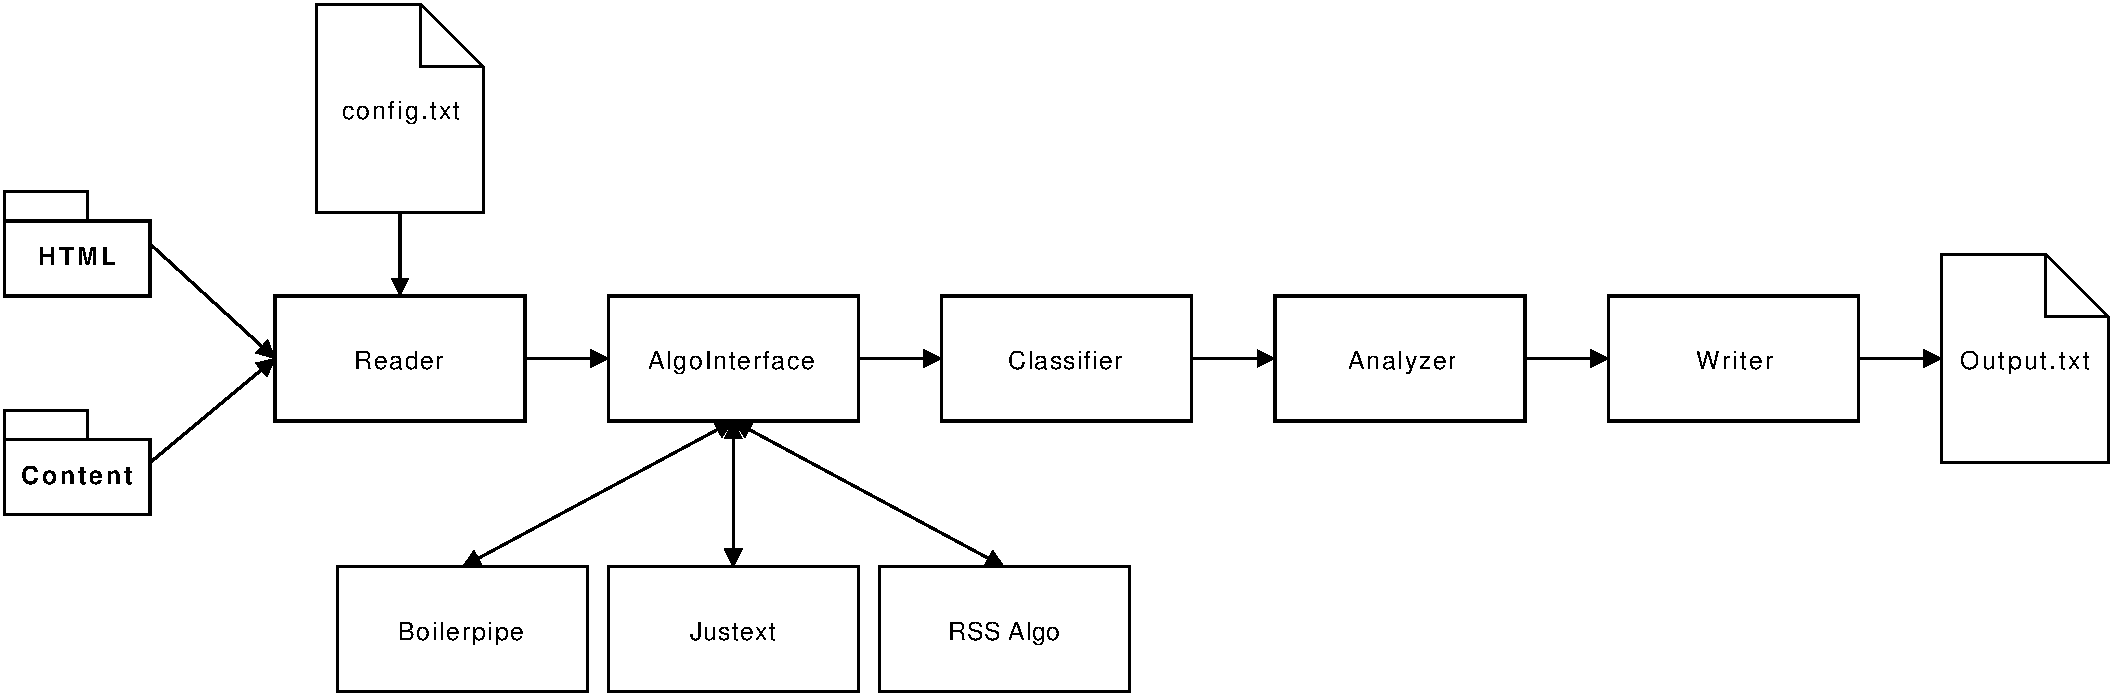
\includegraphics[width=24cm]{Figures/App_overview.pdf}

There are two folders defined by the configuration file (config.txt). The HTML folder contains  HTML files of web pages. The content folder contains text files with the relevant content of the related HTML files. As soon as a test is started, the HTML file and the text file are read and the HTML file is extracted and classified with all the available algorithms. The result of the classification is then compared to the relevant content and performance data is generated. This performance data is then analyzed with statistical methods. 

\end{landscape}



\subsection{Overview}

	\begin{tabular}{ | p{0.5cm} | p{9cm} |p{2cm} |p{2.5cm} |}
	\hline
	\textbf{ID}	& \textbf{Name} 									& \textbf{Chapter}    											& \textbf{Relevance}	\\ \hline
	f1  		& Read configuration 								& \ref{subsec:Read configuration}  								& needed 				\\ \hline
	f2  		& Create test 										& \ref{subsec:Create test}										& needed 				\\ \hline
	f3  		& Integration Justext algorithm 					& \ref{subsec:Integration Justext algorithm} 					& needed 				\\ \hline
	f4  		& Integration Boilerpipe algorithm 					& \ref{subsec:Integration Boilerpipe algorithm}  				& needed 				\\ \hline
	f5  		& Evaluation and Implementation RSS feed algorithm 	& \ref{subsec:Evaluation and Implementation RSS feed algorithm} & nice to have			\\ \hline
	f6  		& Evaluation of classification text 				& \ref{subsec:Evaluation of classification text}				& needed 				\\ \hline
	f7  		& Evaluation of classification blocks 				& \ref{subsec:Evaluation of classification blocks}	  			& nice to have			\\ \hline
	f8  		& Analyze data 										& \ref{subsec:Analyze data}										& needed 				\\ \hline
	\end{tabular} \\



\subsubsection{Read configuration}
\label{subsec:Read configuration}

	\begin{tabular}{ | p{3cm} | p{12cm} |}
	\hline
	\textbf{Name} 				& Read configuration 				\\ \hline
	\textbf{Feature id} 		& f1 				\\ \hline
	\textbf{Description} 		& The text extraction framework is configurable with an external text file. The configuration file will contain following items:
							        \begin{itemize}
							        \item Path to folder with HTML files
							        \item Path to folder with text files
							        \item Path to folder with output files
							        \item Configuration for algorithms
							        \item etc.
						        \end{itemize} 
						        The configuration file location is defined as a relative path to the source directory and structured in a key value list: 

						        \lstinputlisting{Code/config_template.txt} \\ \hline
	\textbf{Relevance} 			& needed 			\\ \hline
	\textbf{Related stories} 	& tbd		\\ \hline
	\end{tabular} \\

\subsubsection{Create test}
\label{subsec:Create test}

	\begin{tabular}{ | p{3cm} | p{12cm} |}
	\hline
	\textbf{Name} 				& Create test \\ \hline
	\textbf{Feature id} 		& f2 \\ \hline
	\textbf{Description} 		& A test contains two input files which are an HTML file and a text file. They are located in the directories defined by the configuration. As soon as the test framework finds an HTML and a text file with the same name, the files are read and the test is started.\\ \hline
	\textbf{Relevance} 			& needed \\ \hline
	\textbf{Related stories} 	& tbd \\ \hline
	\end{tabular} \\

\subsubsection{Integration Justext algorithm}
\label{subsec:Integration Justext algorithm}

	\begin{tabular}{ | p{3cm} | p{12cm} |}
	\hline
	\textbf{Name} 				& Integration Justext algorithm \\ \hline
	\textbf{Feature id} 		& f3 \\ \hline
	\textbf{Description} 		& Justext is implemented in python. That is the reason why a service is needed to call the python script and get the extracted text or the extracted blocks.\\ \hline
	\textbf{Relevance} 			& needed \\ \hline
	\textbf{Related stories} 	& tbd \\ \hline
	\end{tabular} \\

\subsubsection{Integration Boilerpipe algorithm}
\label{subsec:Integration Boilerpipe algorithm}

	\begin{tabular}{ | p{3cm} | p{12cm} |}
	\hline
	\textbf{Name} 				& Integration Boilerpipe algorithm \\ \hline
	\textbf{Feature id} 		& f4 \\ \hline
	\textbf{Description} 		& Boilerplate is implemented in Java. An interfae is needed in order to call the Boilerplate component and get the extracted text or the extracted blocks.\\ \hline
	\textbf{Relevance} 			& needed \\ \hline
	\textbf{Related stories} 	& tbd \\ \hline
	\end{tabular} \\

\subsubsection{Evaluation and Implementation RSS feed algorithm}
\label{subsec:Evaluation and Implementation RSS feed algorithm}

\begin{tabular}{ | p{3cm} | p{12cm} |}
	\hline
	\textbf{Name} 				& Evaluation and implementation RSS feed algorithm \\ \hline
	\textbf{Feature id} 		& f5 \\ \hline
	\textbf{Description} 		& The basic idea of the RSS feed algorithm is to match the content of an HTML document with the related RSS feed and in doing so, define the relevant content. This needs to be evaluated, implemented and integrated into the text extraction framework.  \\ \hline
	\textbf{Relevance} 			& nice to have\\ \hline
	\textbf{Related stories} 	& tbd \\ \hline
	\end{tabular} \\

\subsubsection{Evaluation of classification text}
\label{subsec:Evaluation of classification text}

	\begin{tabular}{ | p{3cm} | p{12cm} |}
	\hline
	\textbf{Name} 				& Evaluation of classification \\ \hline
	\textbf{Feature id} 		& f6 \\ \hline
	\textbf{Description} 		& All the text extraction algorithms return an extracted document as text. This document needs to be checked for accuracy, which is achieved by comparing the result of the algorithms with the actual content. 
								\begin{itemize}
							        \item Check each classified block from the algorithms if its content can be found in the actual content
							        \item Categorize text as boilerplate or content
							        \item Insert results in an output text file
						        \end{itemize} 

						        Both the evaluation and classification are defined in more detail in section \ref{subsec:Evaluation of classification}.
						        \\ \hline

	\textbf{Relevance} 			& needed\\ \hline
	\textbf{Related stories} 	& tbd \\ \hline
	\end{tabular} \\


\subsubsection{Evaluation of classification blocks}
\label{subsec:Evaluation of classification blocks}

	\begin{tabular}{ | p{3cm} | p{12cm} |}
	\hline
	\textbf{Name} 				& Evaluation of classification blocks \\ \hline
	\textbf{Feature id} 		& f6 \\ \hline
	\textbf{Description} 		& A more detailed evaluation of the algorithms could be done if not only the text but also each block of an HTML file is classified. So as to achieve the more detailed evaluation, the implementation of Justext and Boilerpiple has to be adapted so that they return classified blocks instead of the extracted text. These blocks are afterwards compared with the actual content and classified. 
								\begin{itemize}
							        \item Check each classified block from the algorithms if its content can be found in the content file
							        \item Categorize all blocks as boilerplate or content
							        \item Insert the results in an output text file (structure output file: tbd)
						        \end{itemize} 
	Both the evaluation and classification are defined in more detail in section \ref{subsec:Evaluation of classification}.
	\\ \hline
	\textbf{Relevance} 			& nice to have\\ \hline
	\textbf{Related stories} 	& tbd \\ \hline
	\end{tabular} \\





\subsection{Analyze data}
\label{subsec:Analyze data}

	\begin{tabular}{ | p{3cm} | p{12cm} |}
	\hline
	\textbf{Name} 				& Analyze data \\ \hline
	\textbf{Feature id} 		& f7 \\ \hline
	\textbf{Description} 		&  From the results of the comparison further values can be evaluated for a better understanding of the results. These values are described in more detail in section \ref{subsec:Analytical values}.
								    \\ \hline
	\textbf{Relevance} 			& needed \\ \hline
	\textbf{Related stories} 	& tbd \\ \hline
	\end{tabular} \\

\subsection{Evaluation of classification}
\label{subsec:Evaluation of classification}


The general meaning of the expressions true positive, true negative, false positive and false negative related to the text extraction topic is shown in following table.

\begin{table}[h]
\begin{tabular}{|p{4cm} |p{5.5cm} |p{5.5cm} |}\hline
          								& \textbf{Classified as content} 	& \textbf{Classified as boilerplate} 	\\ \hline
\textbf{Actual content} 				& True positive (TP)				& False negative(FN)					\\ \hline
\textbf{Actual boilerplate} 			& False positive (FP)       		& True negative (TN)				 	\\ \hline
\end{tabular}
\end{table}

When the results are compared based on words, the expressions are interpreted as follows.

 \begin{table}[h]
\begin{tabular}{|p{4cm} |p{5.5cm} |p{5.5cm} |}
\hline         								& \textbf{Classified as content} 				& \textbf{Classified as boilerplate} 					\\ \hline
\textbf{Actual content} 				& Word classified as content by algorithm and is content		& Word classified as content by algorithm but is boilerplate		\\ \hline
\textbf{Actual boilerplate} 			& Word classified as content by algorithm but is boilerplate 	& Word classified as boilerplate by algorithm and is Boilerplate	\\ \hline
\end{tabular}
\end{table}

When the results are compared based on HTML blocks, the expressions are interpreted as follows.

 \begin{table}[h]
\begin{tabular}{|p{4cm} |p{5.5cm} |p{5.5cm} |}
\hline         							& \textbf{Classified as content} 								& \textbf{Classified as boilerplate} 								\\ \hline
\textbf{Actual content} 				& Block is classified as content by algorithm and is content		& Block is classified as content by algorithm but is boilerplate		\\ \hline
\textbf{Actual boilerplate} 			& Block is classified as content by algorithm but is boilerplate 	& Block is classified as boilerplate by algorithm and is boilerplate	\\ \hline
\end{tabular}
\end{table}

In conclusion, TP + FN is the correct outcome of the algorithm i.e. content classified as content and boilerplate as boilerplate. On the other hand, TN + FP is the wrong outcome of the algorithm i.e. content classified as boilerplate and boilerplate as content.



\subsection{Analytical values}
\label{subsec:Analytical values}

In this paragraph we use the notion of objects instead of word/block.
The results of the comparison deliver basic characteristics which can be used to calculate statistical values which help you analyze the test outcome.
										
\textbf{ Sensitivity / Recall /True positive rate / TPR / Hitrate }

Recall is the probability that a relevant document is retrieved in a search which in our case is

\begin{equation}
 Recall =\frac{TP}{TP + FN}
\end{equation}

correct classified content objects divided by the sum of all actual objects.

\textbf{Precision / True negative rate / TNR} 


Precision is the probability that a retrieved document is relevant which in our case is

\begin{equation}
 Presicion = \frac{TP}{TP + FP}
\end{equation}

correct classified content objects divided by the sum of all objects classified as content.

\textbf{F-measure / F1-score / F-score} 

F-measure is the harmonic mean of precision and recall which in our case is

\begin{equation}
Fmeasure =  2* \frac{presicion * recall}{presicion + recall}
\end{equation}

a measure of the test's accuracy.



\textbf{Fallout / False positive rate / FPR}

Fallout is the proportion of non-relevant objects that are retrieved out of all non-relevant objects available which in our case is

\begin{equation}
Fallout = \frac{FP}{FP + TN}
\end{equation}

%\textbf{Accuracy}

%\begin{equation}
%Accuracy =  \frac{TP+FN}{TP+TN+FP+FN}
%\end{equation}


\section{External Interface Requirements}

\subsection{Boilerpipe}

The boilerpipe algorithm is implemented in Java and the documentation is found under
\url{https://code.google.com/p/boilerpipe/}.

\subsection{justext}

The justext algorithem is implemented in python and the documentation is found under \url{https://code.google.com/p/justext/}. It is not yet defined how it will be integrated into the text extraction framework. See risk analysis for further information.



% Chapter Template

\chapter{Software Architecture} % Main chapter title

\label{architecture} % Change X to a consecutive number; for referencing this chapter elsewhere, use \ref{ChapterX}

\lhead{\emph{Software Architecture}} % Change X to a consecutive number; this is for the header on each page - perhaps a shortened title

%----------------------------------------------------------------------------------------
%	SECTION 1
%----------------------------------------------------------------------------------------

\section{Version}

\begin{tabular}{| p{1.5cm} | p{2cm} | p{9cm} | p{1.5cm} |}
	\hline
	Version & Date 		& Change & Author \\ \hline
	0.1 	& 8.10.2014 		& Setup document  										& JR \\ \hline
	0.2 	& 12.10.2014		& Class diagrams										& JR \\ \hline
	0.3 	& 16.10.2014		& Text													& JR \\ \hline
	0.4 	& 20.10.2014		& Activity diagram										& JR \\ \hline
	1.0 	& 21.10.2014		& Grammar, Diagram fixes								& JR \\ \hline
	1.1 	& 22.10.2014		& Adding description of all business logic classes, approach and extended introduction & JR \\ \hline
	1.2 	& 23.10.2014		& Grammar & JR,LR \\ \hline

\end{tabular}

\section{Introduction} 

This document describes the software architecture of the context extraction test framework. 
The context extraction test framework will perform automated text extraction on a set of HTML test data with two to three different text extraction algorithms. After measuring the performance of each algorithm, an output file with the measured results is generated.

\section{System Overview}

This section describes the approach for elaborating the software architecture and gives an overview over the software architecture. 
The following figure from the software requirement specification is the basis for elaborating the software architecture.

%\begin{landscape}
\ref{asfdsafdsa}
\begin{figure}
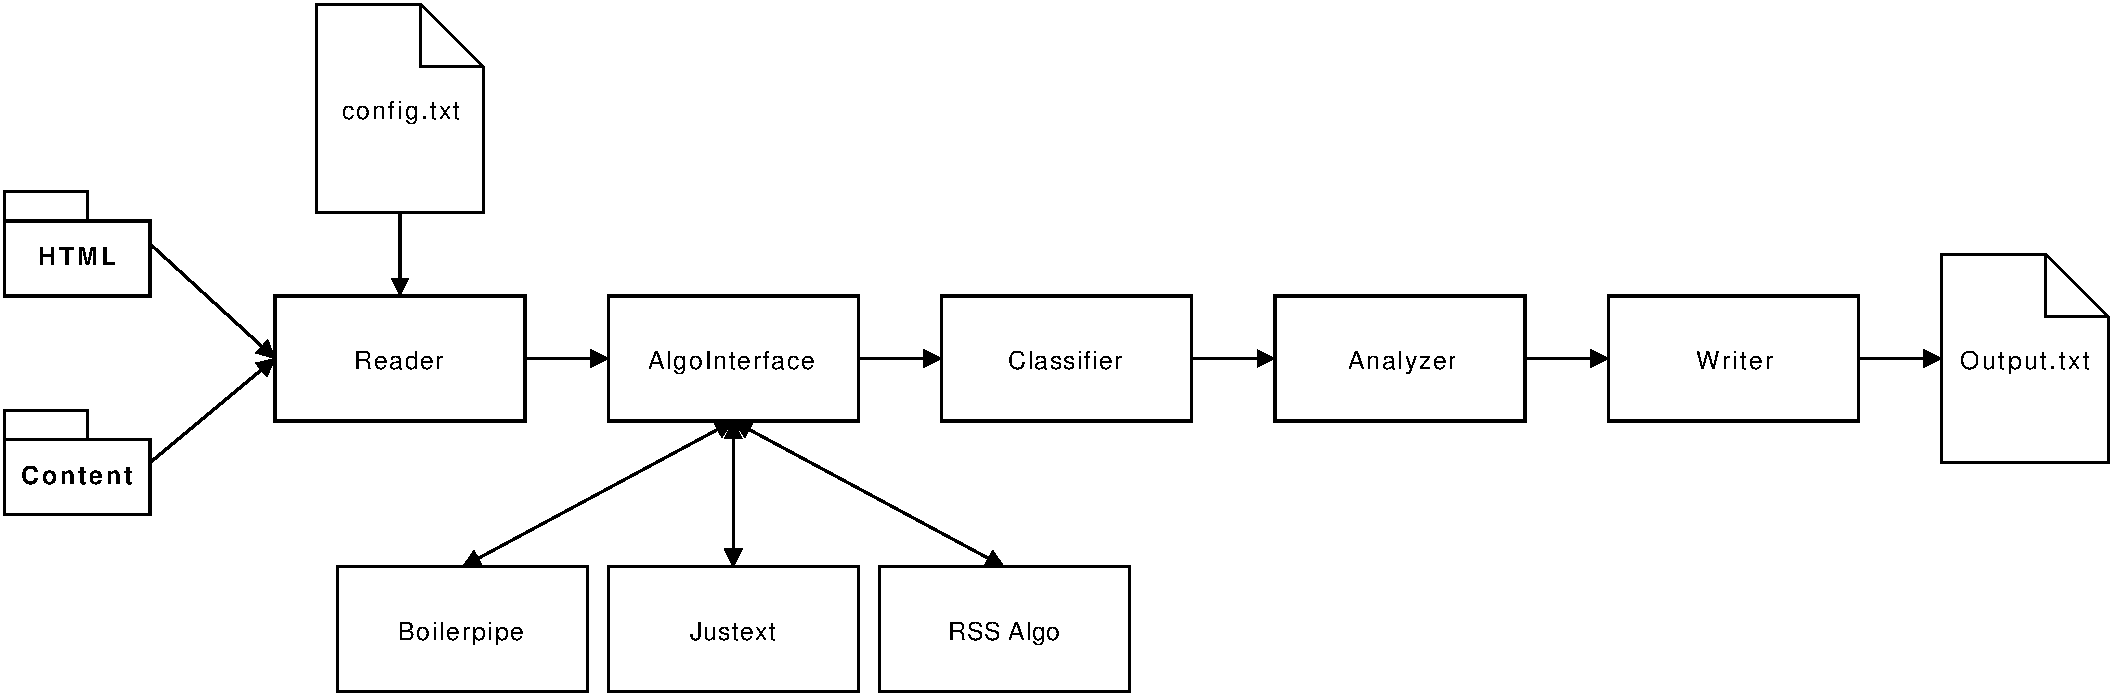
\includegraphics[width=15cm]{Figures/AppOverview.pdf}
\caption{blablalb}
\label{asfdsafdsa}
\end{figure}
%\end{landscape}

First all possible entities in the domain are identified and a data model is elaborated. The data model is described in section \ref{subsec:Data model}. Then the business logic is researched based on the figure above. With this knowledge, the five packages main, reader, classifier, analyzer and writer are defined. The functions for each package is then evaluated and split into single classes. During the implementation of the first approach, some classes are adapted due to unforeseen circumstances. The outcome is described in section \ref{subsec:Business Logic}.
\pagebreak

\section{Logical view}

This section describes how the system is structured in terms of units of implementation.


\subsection{Data model}
\label{subsec:Data model}

The following diagram shows the data model of the application. 

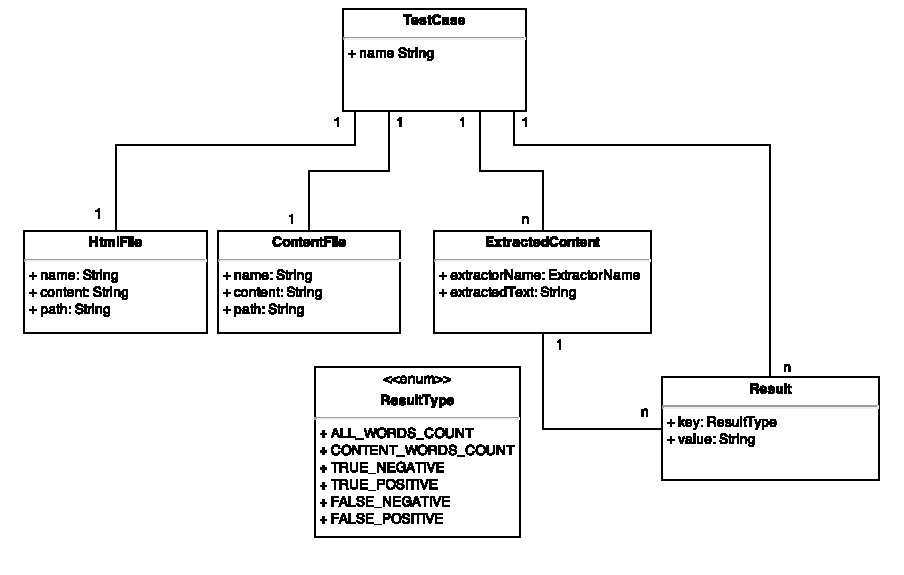
\includegraphics[width=14cm]{Figures/dataModel.pdf}


\subsection{TestCase}
A TestCase object is generated for each HTML/content file pair in the input folders. A TestCase has a a name which is unique and which matches the name of the content and HTML file.

\subsection{HtmlFile}
Each TestCase has an HtmlFile object. It contains the content of the actual HTML file as String and the file path.

\subsection{ContentFile}
Each TestCase has a ContentFile object. It contains the content of the actual text file as String and the file path.

\subsection{ExctractedContent}
Each TestCase can have multiple ExctractedContent objects. Each of them represents a result of a content extraction from an extractor such as JusText or Boilerpipe. It contains the extracted text as well as the extracted text separated in Block objects with the generated classification.

\subsection{Result}
A TestCase or an ExctractedContent object can have Result objects. The results are key value pairs which represent analytical data. An example for a Result related to a TestCase would be the word count of the content file, which is generally valid. An example for a Result related to an ExctractedContent would be the word count of true negative words, which is only valid for one specific ExctractedContent.

\subsection{Config}
A Config object contains all configurable information about a test run. It is generated from the config.txt file at the beginning of the test. Configuration parameters like test language, used extractors, possible filters are defined by the Config object.
\begin{landscape}

\subsection{Business Logic}
\label{subsec:Business Logic}

The following diagram shows the business logic of the application. The diagram does not show all of the classes but the most important ones. 

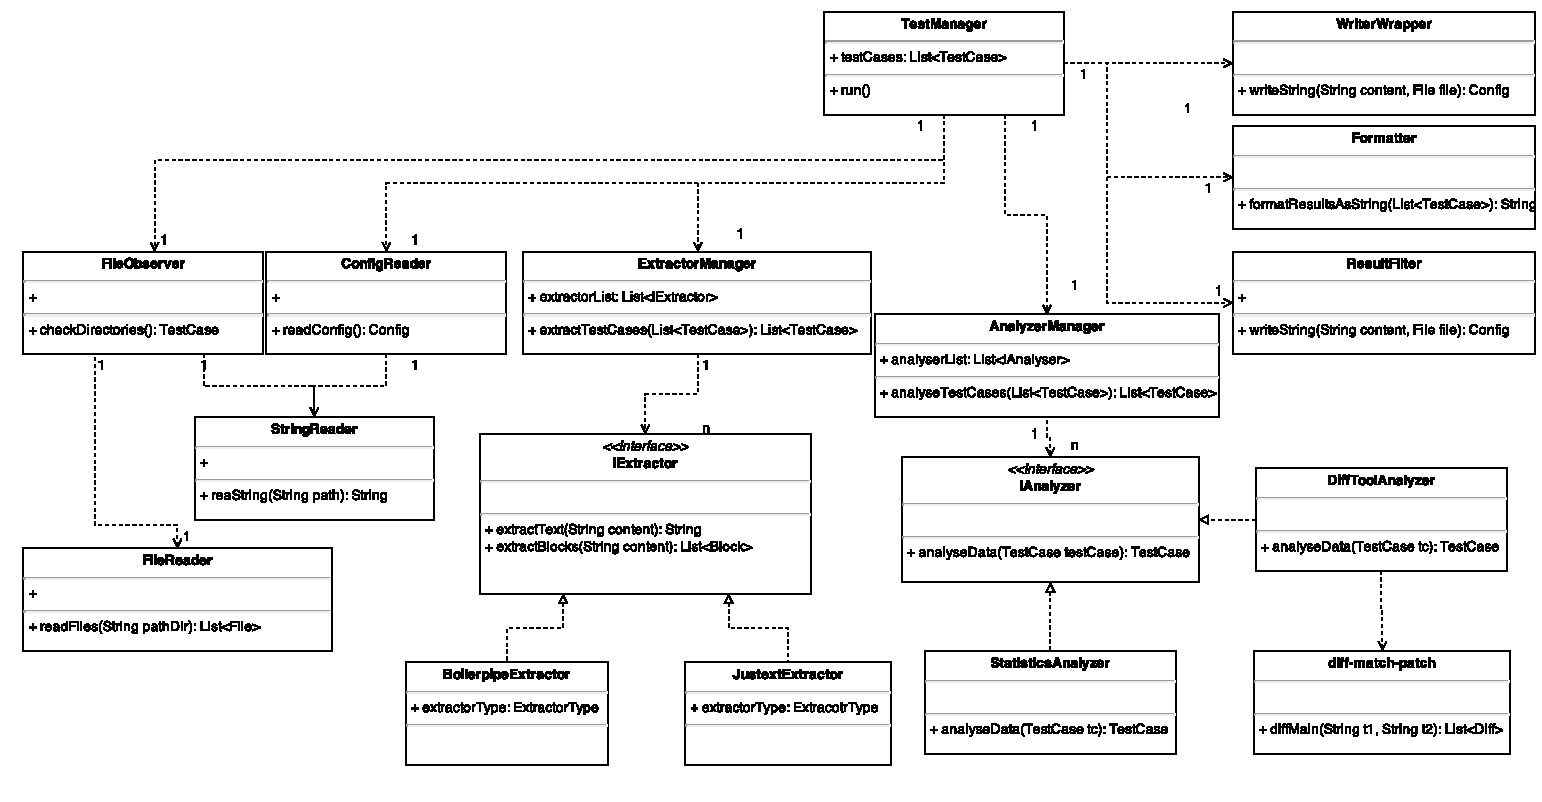
\includegraphics[width=23cm]{Figures/architecutre.pdf}


\end{landscape}



\pagebreak
\subsection{Description of single classes}

\begin{longtable}{p{4cm}|p{2cm}|p{8cm}}
\hline
\textbf{Class} &
\textbf{Package} &
\textbf{Description}
 \\ \hline
TestManager &
testManager &
The TestManager class manages the whole business logic that manages TestCase objects through the whole test process from reading the file content to writing the test results into an output file.
 \\ \hline
FileObserver &
reader &
The FileObserver class checks the HTML and content directory for files of the same name and creates TestCases from each found pair. The folders are checked with the FileReader class and the content of the files are read with the StringReader class.
\\ \hline
StringReader &
reader &
The StringReader class reads a text file and returns the content as String. The class is made for easier mocking of the BufferedReader so that testing of other classes which are dependent on external files becomes much easier.
\\ \hline
FileReader &
reader &
The FileReader class returns a File objects for each found file in a directory given by a parameter.
\\ \hline
ExtractorManager &
classifier &
The ExtractorManager manages all available Extractors. Each extractor which is used for the actual test must be initialized in this class and added to the ExtractorList. Each TestCase is then extracted by every IExtractor in the ExtractorList.
\\ \hline
IExtractor &
classifier &
The IExtractor is the interface to the different extractor. The interface is very lightweight. The parameter is the text that should be extracted and the return value is the extracted text.
\\ \hline
BoilerpipeExtractor &
classifier &
The BoilerpipeExtractor implements the IExtractor and is the interface to the Boilerpipe package. It handles all dependencies on the Boilerpipe package and returns the extracted content as a string.
\\ \hline
JusTextExtractor &
classifier &
The BoilerpipeExtractor implements the IExtractor and is the interface to the JusText python program. The Java ProcessBuilder is used to create operating processes. One can then perform operating system commands and run the python script. The python script creates a text file with the extracted content which is read by the JusTextExtractor class and returned as String.
\\ \hline
AnalyzerManager &          
analyzer &          
The AnalyzerManager manages all available analyzers. Each analyzer which is used for the actual test must be initialized in this class and added to the AnalyzerList. Each TestCase is then analyzed by every IAnalyzer in the AnalyzerList.
\\ \hline
IAnalyzer &
analyzer &
The IAnalyzer interface is a simple interface to the different analyzers. Each analyzer can generate one or more Result objects.
\\ \hline
DiffToolAnalyzer &
analyzer &
The DiffToolAnalyzer compares two Strings and generates the values TP, FP, TN and FN and puts them as Result object into the test cases.
\\ \hline
StatisticsAnalyzer &
analyzer &
The StatisticsAnalyzer extracts the values TP, TN, FP, FN from the test cases and calculates Precision, Recall, F-Measure, Fallout and accuracy and FN and puts them as Result object into the test cases.
\\ \hline
ResultFilter &
writer &
Filters all TestCases for the filters given in the configuration objects.
\\ \hline
Formatter &           
writer &           
The Formatter class formats a string from all TestCase objects as a CSV file structure. This means that a table with the Result keys as table header for each column is created. For each TestCase a row with the Result value field as values is added to the table. The outcome is a CSV file which can easily be imported into another program such as Excel so that one can work with the data.
\\ \hline
WriterWrapper &
writer &
The writer wrapper writes a string into a text file. It is used to wrap the BufferedWriter so that mocking and testing of dependent classes is easier.
\\ \hline
ConfigReader &
reader &
The ConfigReader class reads the config.txt file and generates a Config object. This object contains the test language, the used extractors, possible filters and single test cases which are inspected for closer inspection.
\\ \hline
\end{longtable}


\section{Process view}

This section describes the dynamic aspects of the application.

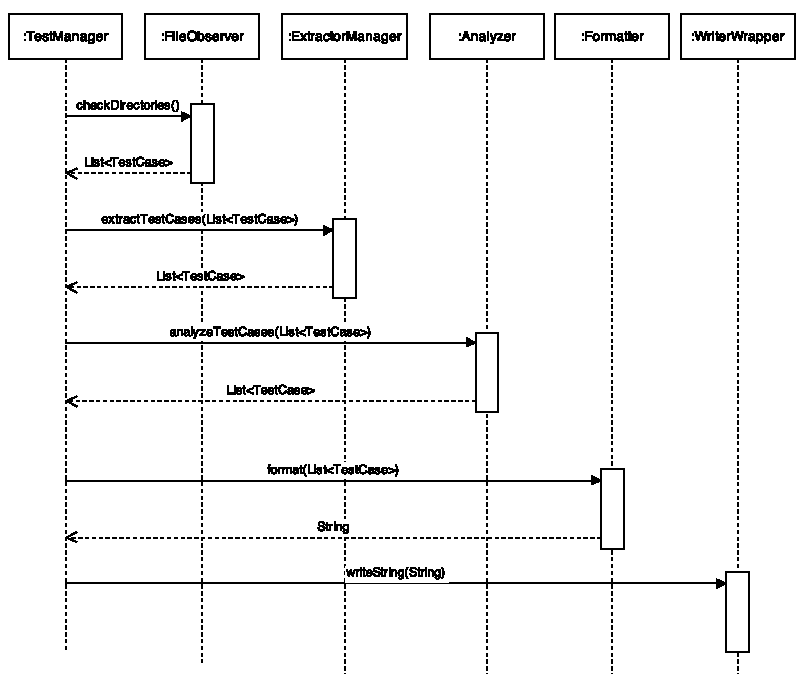
\includegraphics[width=15cm]{Figures/activityDiagram.pdf}

The data model is passed through the business logic and is enriched with data during the test procedure. First the input directories are checked for files by the FileObserver and TestCases are generated for each file pair with the same name. Then all the TestCases are then handed over to the ExtractorManager. The ExtractorManager extracts each TestCase with all available implementations of IExtractor and puts the Results into ExtractionResults. After that, all the TestCases are handed over to the Analyzer which runs each implementation of IAnalyzer. Each IAnalyzer produces at least one Result and puts it into the TestCase. To simplify the diagram, only two Analyzers are drawn. After generating the Results, they are filtered if any filter is set in the Config object. Then, the Formatter serializes the Result Objects into a String as a CSV table and the WriterWrapper persists the CSV data into an output file.


\section{Development view}
\label{architecture:developmentView}

This chapter describes the used tools and libraries which are used during the development process as well as the continuous integration process.


\subsection{Continuous Integration Process}

The continuous integration process for this process is handled with the version control tool Git, the continuous integration server Travis CI and the project automation tool Gradle. The single tools are described in more details in the following sections. The general process is however defined like this. Since this is a one man project, there is only one Git branch present for the most time of the development phase. The application is developed on the local branch and unit tests are written for critical components. The application is then built locally with Gradle. Possible problems are solved and the changes are pushed on the master Git repository. As soon as there are any new commits on the master repository, the application is built as well on the Travis CI server. If the build is not successful. An error report is sent to the user.

\subsection{Git}

Git is a distributed version control system. Unlike other version control systems like Subversion, Git is not using a central server but each user has his own copy with the complete history on the local system. It is much easier to work with additional branches or tags. 
Because of these advantages and because Layzapp is working with it as well, Git was chosen to use for this project for the code sources and as well for the documentation.
The resources are open source and are available under following links.

\begin{itemize}
\item code: \url{https://Github.com/heya87/pawiTwo}
\item documentation: \url{https://Github.com/heya87/pawi_doc}
\end{itemize}


\subsection{Gradle}

Gradle is a project automation tool which uses a Groovy-based domain-specific language (DSL) instead of the more traditional XML form of declaring the project configuration. All the dependencies of the project are handled with Gradle and it is very easy to deploy on a new system. The user only needs to download the Git repository and can build the project with the Gradle wrapper without installing any new software. All dependencies are then downloaded automatically and the user can start working without caring about missing packages.
The build process is defined in the build.gradle file which is located in the source directory of the project. 

\subsection{Travis CI}

Travis CI is an open source build server. It is easy to use in combination with Git. One only needs to add a configuration file in the source directory of the project and define the Git repository. Afterwards the project is build for every change. If the build does not pass, a mail is sent to the user. The actual status of the build can be found under following link \url{https://travis-ci.org/heya87/pawiTwo}.

\subsection{JusText}

An implementation of the JusText algorithm is available in Python. The resources are available under following link \url{https://code.google.com/p/justext/}. There is no implementation in Java so for the first approach the python application is called from Java with a ProcessBuilder.
The command to extract an HTML file with JusText is very simple:

\begin {lstlisting}
justext -s English /path/page.html > cleaned-page.txt
\end{lstlisting}

This command extracts the HTMl file page.html into a text file called cleaned-page.txt. The Java ProcessBuilder performs system commands as they are used in a console and can handle the outcome if needed. For the project there is no return values needed. The needed content is the generated text file which is then read and processed for further use.

\subsection{Boilerpipe}

An implementation of the Boilerpipe Algorithm is available in Java. The resources are available under following link \url{https://code.google.com/p/boilerpipe/}. This algorithm can be used out of the box with calls against the Java API.

\subsection{diff-match-patch}

The Java library diff-match-patch \cite{google:diffMatchPatch} is used to compare text files and find differences. For this file, it is used to extract the values TP, TN, FP, FN when comparing the actual content files with the outcome of the algorithms.


\section{Physical view}

Following diagram shows the physical view of the application. The application is running on a single device, which results in a very simple diagram. The external components are the Boilerpipe algorithm implemented in Java and the JusText algorithm implemented in Python. The python program is called with system calls. All the components are located on the same device. 
The config.txt file contains configuration parameter for the application and the different output text files contain the results of the test framework.

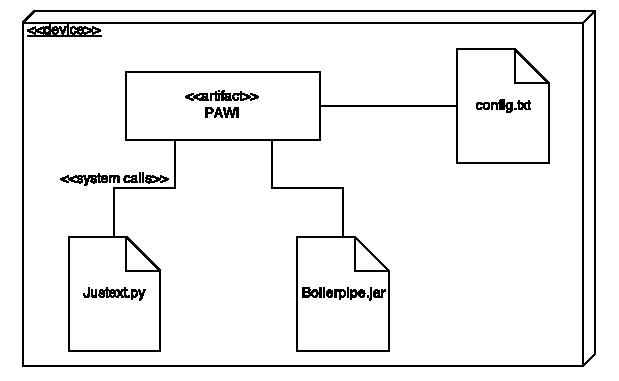
\includegraphics[width=10cm]{Figures/deploymentDiagram.pdf}



% Chapter 2

\chapter{Test plan} % Main chapter title

\label{Test plan} % For referencing the chapter elsewhere, use \ref{Chapter1} 

\lhead{Test plan} % This is for the header on each page - perhaps a shortened title

%----------------------------------------------------------------------------------------

\section{Introduction}


\subsection{Test concept}

The project was tested on two levels. The first level is Unit Testing in Java. This tests are not documented in the report itself. Since the project was developed in a continuous integration environment, all unit tests were run after committing any changes to the git repository. If any test did not pass, the build would fail. With this functionality, the most important and critical functions of the functionalities are already covered. The continuous integration environment is described in the system requirement specification (\ref{Software Requirement Specification}). \linebreak 
However the second level are test cases which are defined against the software requirement specification and are performed as blackbox test.  To do so, test cases were defined so they cover all the features defined in the software requirement specification. 

\subsection{Test cases}

This section contains all test cases which cover the features described in the software requirement specification. The results of the single test runs can be found in the test protocol (\ref{Test protocol}).


	\begin{tabular}{ | p{3.5cm} | p{12cm} |}
	\hline
	\textbf{Name} 					& Test case handling 	\\ 	\hline
	\textbf{Test case id} 			& tc1 					\\ 	\hline
	\textbf{Description} 			& Create 10 tests and check the detailed output file for the right amount of tests. 	\\ 	\hline
	\textbf{Related features}		& f2		\\ 	\hline
	\textbf{Test steps} 			& 	\begin{enumerate}
											\item{Put ten text files into the content input folder.}
											\item{Put ten html files into the html input folder. They need to have the same name as the related content files.}
											\item{Run the test}
										\end{enumerate}
										\\ 	\hline
	\textbf{Preconditions} 			& At least one extractor needs to be activated in the config file.	\\ 	\hline
	\textbf{Preconditions} 			& An output file \'output\_detailed.txt\' needs to be created. The text file needs to contain exactly ten result lines, for each 											test one line. The tests need to be named the same as the input files in the content resp. the html folder.	\\ 	\hline
	\end{tabular} \\


	\begin{tabular}{ | p{3.5cm} | p{12cm} |}
	\hline
	\textbf{Name} 					& Config single test		\\ 	\hline
	\textbf{Test case id} 			& tc2 						\\ 	\hline
	\textbf{Related features}		& f1, f2						\\ 	\hline
	\textbf{Description} 			& The detailed results for a single test need to be put into an extra output file when it is defined in the config file. \\ 	\hline
	\textbf{Test steps} 			& 	\begin{enumerate}
											\item{Add following line to the config file: "inspect:testToInspect" where testToInspect is a file name of any content/HTML file pair in the input folder. }
											\item{Run the test}
											\item{Check the outputfolder for following file: "result\_testToInspect.txt"}
										\end{enumerate}
																\\ 	\hline
	\textbf{Preconditions} 			& tc1 needs to be fulfilled							\\ 	\hline
	\textbf{Acceptance criteria} 	& A file with the name "result\_testToInspect.txt" is present in the output folder. \\ 	\hline
	\end{tabular} \\


	\begin{tabular}{ | p{3.5cm} | p{12cm} |}
	\hline
	\textbf{Name} 					&  Run the boilerpipe algorithm with the test framework\\ 	\hline
	\textbf{Test case id} 			& tc3 						\\ 	\hline
	\textbf{Related features}		& f4 						\\ 	\hline
	\textbf{Description} 			& Check if the test framework is working with the boilerpipe algorithm.	\\ 	\hline
	\textbf{Test steps} 			& 	\begin{enumerate}
											\item{Add any content/HTML file pair into the input folders.}
											\item{Add following line into the config file: "extractor:boilerpipe"}
											\item{Run the test}
											\item{Check the output files for results produced for the boilerpipe extractor.}
										\end{enumerate}
																\\ 	\hline
	\textbf{Preconditions} 			& tc1/tc2 need to be fulfilled 							\\ 	\hline
	\textbf{Acceptance criteria} 	& The outputfile output.txt needs to have results for the boilerpipe extractor.\\ 	\hline
	\end{tabular} \\



	\begin{tabular}{ | p{3.5cm} | p{12cm} |}
	\hline
	\textbf{Name} 					&  Run the Justext algorithm with the test framework\\ 	\hline
	\textbf{Test case id} 			& tc4 						\\ 	\hline
	\textbf{Related features}		& f3						\\ 	\hline
	\textbf{Description} 			& Check if the test framework is working with the Justext algorithm.	\\ 	\hline
	\textbf{Test steps} 			& 	\begin{enumerate}
											\item{Add any content/HTML file pair into the input folders.}
											\item{Add following line into the config file: "extractor:justext"}
											\item{Run the test}
											\item{Check the output files for results produced for the Justext extractor.}
										\end{enumerate}
																\\ 	\hline
	\textbf{Preconditions} 			& tc1/tc2 need to be fulfilled 							\\ 	\hline
	\textbf{Acceptance criteria} 	& The output file output.txt needs to have results for the Justext extractor.\\ 	\hline
	\end{tabular} \\

	\begin{tabular}{ | p{3.5cm} | p{12cm} |}
	\hline
	\textbf{Name} 					& Test analysis 		 		\\ 	\hline
	\textbf{Test case id} 			& tc5 							\\ 	\hline
	\textbf{Related features}		& f6, f8							\\ 	\hline
	\textbf{Description} 			& Run a test with one test file and check the results (TP, TN, FP, FN). To do so, run a detailed test (needs to be defined in the config file) for the according test and check the results by hand. The contains the actual content file as well as the extracted files by the algorithms. This output file can be used to check the results. 	\\ 	\hline
	\textbf{Test steps} 			& 	\begin{enumerate}
											\item{Put an HTML file into the HTML input folder.}
											\item{Put an according content file into the content input folder.}
											\item{Add following line into the config file: "inspect:testToInspect" where "testToInspect" accords to the name of the test files.}
											\item{Run the test}
											\item{Open the file results\_testToInspect.txt}
											\item{Check the values for TP, TN, FP, FN by hand}
										\end{enumerate}
																\\ 	\hline
	\textbf{Preconditions} 			& tc2 needs to be fulfilled	\\ 	\hline
	\textbf{Acceptance criteria} 	& The results in the output file for TP, TN, FP, FN need to be correct.						\\ 	\hline
	\end{tabular} \\





	\begin{tabular}{ | p{3.5cm} | p{12cm} |}
	\hline
	\textbf{Name} 					& Evaluation of Precision, Recall, F-Measure, Fallout 		\\ 	\hline
	\textbf{Test case id} 			& tc6 						\\ 	\hline
	\textbf{Related features}		& f6, f8						\\ 	\hline
	\textbf{Description} 			& Check the calculated values  Precision, Recall, F-Measure and Fallout for any test case.	\\ 	\hline
	\textbf{Test steps} 			& 	\begin{enumerate}
											\item{Put any test file pair into the input folders.}
											\item{Add following line into the config file: "inspect:testToInspect" where "testToInspect" accords to the name of the test files. }
											\item{Open the file test\_testToInspect.txt.}
											\item{Calculate the values for Precision, Recall, F-Measure and  Fallout from the TP, FP, TN, FN values and compare them with the values in the output file.}
										\end{enumerate}
																\\ 	\hline
	\textbf{Preconditions} 			& tc1, tc5							\\ 	\hline
	\textbf{Acceptance criteria} 	& The values Precision, Recall, F-Measure and Fallout need to be calculated correctly.	\\ 	\hline
	\end{tabular} \\




	\begin{tabular}{ | p{3.5cm} | p{12cm} |}
	\hline
	\textbf{Name} 					& Block data evaluation 		\\ 	\hline
	\textbf{Test case id} 			& tc7						\\ 	\hline
	\textbf{Related features}		& f7						\\ 	\hline
	\textbf{Description} 			& Check that the detailed results contains the classification information from each algorithm.	\\ 	\hline
	\textbf{Test steps} 			& 	\begin{enumerate}
											\item{Put any test file pair into the input folders.}
											\item{Add following line into the config file: "inspect:testToInspect" where "testToInspect" accords to the name of the test files. }
											\item{Open the file test\_testToInspect.txt.}
											\item{Check for the block information}
										\end{enumerate}
																\\ 	\hline
	\textbf{Preconditions} 			& tc1, tc3, tc4				\\ 	\hline
	\textbf{Acceptance criteria} 	& The detailed output file for one test needs to contain the classification information for each block the algorithms classified.	\\ 	\hline
	\end{tabular} \\
\chapter{Test protocol} % Main chapter title

\label{Test protocol} % For referencing the chapter elsewhere, use \ref{Chapter1} 

\lhead{Test protocol} % This is for the header on each page - perhaps a shortened title

%----------------------------------------------------------------------------------------

\section{Version}

\begin{tabular}{| p{1.5cm} | p{2cm} | p{9cm} | p{1.5cm} |}
    \hline
    Version & Date      & Change & Author \\ \hline
    0.1     & 20.10.2014        & Setup document                                        & JR \\ \hline
    0.2     & 24.10.2014        & Add test run one                                        & JR \\ \hline
    0.3     & 25.11.2014        & Add test run two                                        & JR \\ \hline
    0.4     & 8.12.2014        & Add test run two                                        & JR \\ \hline
    1.0     & 14.12.2014        & Grammar / Formatting                                        & JR \\ \hline
\end{tabular}


\section{Introduction}

This section contains the results of the black box test which were made three times during the projects. The test cases are described in the test plan (\ref{Test plan}). Each test case was tested as described and the results were checked and documented. All the three test runs are documented below.

	\subsection{Test run one}

	\begin{itemize}
	\item Date: 24.10.2014
	\item Test engineer: Joel Rolli 
	\end{itemize}	


	\begin{tabular}{ | p{3cm} | p{2cm} | p{7cm} |}
	\hline
	\textbf{Test case id} 					& \textbf{Restult} & \textbf{Comment} 		\\ 	\hline
	tc1 & pass & - \\ \hline	
	tc2 & pass & - \\ \hline	
	tc3 & fail & only prototype working \\ \hline	
	tc4 & fail & only prototype working \\ \hline	
	tc5 & fail & Working in general but the results are not very exact (comparison is done based one single word counting) \\ \hline	
	tc6 & fail & not implemented \\ \hline	
	\end{tabular} \\


	\subsection{Test run two}

	\begin{itemize}
	\item Date: 25.11.2014
	\item Test engineer: Joel Rolli 
	\end{itemize}	


	\begin{tabular}{ | p{3cm} | p{2cm} | p{3cm} |}
	\hline
	\textbf{Test case id} 					& \textbf{Restult} & \textbf{Comment} 		\\ 	\hline
	tc1 & pass & - \\ \hline	
	tc2 & pass & - \\ \hline	
	tc3 & pass & - \\ \hline	
	tc4 & pass & - \\ \hline	
	tc5 & pass & - \\ \hline	
	tc6 & pass & - \\ \hline	
	\end{tabular} \\


		\subsection{Test run three}

	\begin{itemize}
	\item Date: 8.12.2014
	\item Test engineer: Joel Rolli 
	\end{itemize}	


	\begin{tabular}{ | p{3cm} | p{3cm} | p{3cm} |}
	\hline
	\textbf{Test case id} 					& \textbf{Restult} & \textbf{Comment} 		\\ 	\hline
	tc1 & pass & - \\ \hline	
	tc1 & pass & - \\ \hline	
	tc2 & pass & - \\ \hline	
	tc3 & pass & - \\ \hline	
	tc4 & pass & - \\ \hline	
	tc5 & pass & - \\ \hline	
	tc6 & pass & - \\ \hline	
	tc7 & pass & - \\ \hline	
	tc8 & pass & - \\ \hline	
	\end{tabular} \\
% Chapter 2

\chapter{User manual} % Main chapter title

\label{User manual} % For referencing the chapter elsewhere, use \ref{Chapter1} 

\lhead{User manual} % This is for the header on each page - perhaps a shortened title

%----------------------------------------------------------------------------------------

\section{Introduction}


\section{System requirements}

To use the text extraction test framework, the system needs to fulfill following system requirements.

\begin{tabular}{| p{2cm} | p{1.5cm} | p{9.5cm} |} 
	\hline
	\textbf{Software} & \textbf{Version} & \textbf{Source} \\ \hline
	Ubuntu & 12.04 & \url{http://releases.ubuntu.com/12.04/} \\ \hline
	git & 2.2.0 & \url{http://git-scm.com/download/linux} \\ \hline
	python & 2.7.6 & \url{https://www.python.org/download/releases/2.7.6/} \\ \hline
\end{tabular}


\section{Installation}

\subsection{}
\begin{enumerate}

\item Checkout the repository with git to your favorite directory.
\begin{lstlisting}
git clone https://github.com/heya87/pawiTwo
\end{lstlisting}


\item Use your favorite console application and navigate into the source directory of the checked out repository.

\item Build the project with the gradle wrapper.
\begin{lstlisting}
./gradlew build
\end{lstlisting}



\item Put the test files you would like into the following folders

\item Put the content files into following folder: ~/build/resources/main/content
\item Put the HTML files into following folder: ~/build/resources/main/html
\item Run the test with the gradle wrapper.

\begin{lstlisting}
./gradlew build
\end{lstlisting}
\item Find the results in the output folder: ~/build/resources/main/


\end{enumerate}


\section{Usage \& Configuration}


% Chapter Template

\chapter{Milestone reports} % Main chapter title

\label{Milestone reports} % Change X to a consecutive number; for referencing this chapter elsewhere, use \ref{ChapterX}

\lhead{\emph{Milestone reports}} % Change X to a consecutive number; this is for the header on each page - perhaps a shortened title

%----------------------------------------------------------------------------------------
%	SECTION 1
%----------------------------------------------------------------------------------------

\section{MS 1 report}
\label{reports:ms1report}

\subsection{Introduction}

This document is a short report about the MS1 meeting. The meeting took place on the 1.10.2014.

\subsection{Version}


\begin{tabular}{| p{1.5cm} | p{2cm} | p{9cm} | p{1.5cm} |}
    \hline
    Version & Date      & Change & Author \\ \hline
    1.0    & 1.10.2014        & Setup document / text                                        & JR \\ \hline
    1.1    & 22.10.2014        & forgot Manu!! / grammar / rework                                        & JR \\ \hline
\end{tabular}


\subsection{Attendees}
\begin{itemize}
\item Joel Rolli
\item Michael Kaufmann
\item Patrick Huber
\item Patrik Lengacher
\item Manuel Schneider
\end{itemize}


\subsection{Delivery objects}

\begin{itemize}
\item System specification
\item Sketch software architecture
\item Short presentation CI environment
\item Draft risk evaluation
\end{itemize}

\subsection{Decisions}

The risk evaluation and the CI environment are approved. 
The evaluation of the text extraction was discussed again and it was decided that the evaluation is still done with Words instead of HTML blocks. Doing the evaluation with HTML blocks can still be done but is not part of the PAWI project and would be bonus content. 
Furthermore it was decided that no handmade test data is needed and the data from cleanEval and Gold standard are used for this project.
The draft of the software architecture is ok but needs to be digitalized.
The software architecture needs to be extended with additional data about the analysis of the extracted data. Which means all the formula for TN, FP, TP, FN etc. needs to be defined.


\subsection{Rework}

Following rework needs to be done until the 5.10.2014

\begin{itemize}
\item Extended software specification
\item Digital version of software architecture sketch
\end{itemize}

Update: The listed delivery objects were delivered and approved on the 5.10.2014.


\section{MS2 meeting report}

\subsection{Introduction}

This document is a short report about the MS1 meeting. The meeting took place on the 24.10.2014.

\subsection{Version}


\begin{tabular}{| p{1.5cm} | p{2cm} | p{9cm} | p{1.5cm} |}
    \hline
    Version 	& Date      		& Change & Author 								\\ \hline
    0.1    		& 20.10.2014        & Setup document        				& JR 	\\ \hline
    1.0 		& 27.10.2014 		& add meeting report 					& JR 	\\ \hline
\end{tabular}


\subsection{Attendees}
\begin{itemize}
\item Joel Rolli
\item Michael Kaufmann
\end{itemize}

\subsection{Delivery objects}

\begin{itemize}
\item Elaborated software architecture
\item Tested code of test framework (reader / writer)
\item Interface definition for justext/boilerplate components
\item HTML test data
\end{itemize}


\subsection{Decisions}

All delivery objects are approved. We discussed the text comparison and came to a conclusion that I am going to search for diff tool libraries to do the comparison of text files. Mr. Kaufmann sent me some proposal later on.


\subsection{Rework}

There is no rework to do.
The proposed diff tool libraries are

\begin{itemize}
\item https://code.google.com/p/google-diff-match-patch/
\item https://commons.apache.org/proper/commons-lang/javadocs/api-2.6/org/apache/commons/lang/StringUtils.html
\end{itemize}


The next milestone, which is the implementation of the whole test framework and integration of justext and boilerpipe, is already achieved as well. We decided that MS3 is obsolete and we are going to meet again if there are any ambiguity and if there is not, for MS4.



\section{MS4 meeting report}

\label{ms4report}


\subsection{Introduction}

This document is a short report about the MS4 meeting. The meeting took place on the 21.11.2014.

\subsection{Version}


\begin{tabular}{| p{1.5cm} | p{2cm} | p{9cm} | p{1.5cm} |}
    \hline
    Version 	& Date      		& Change & Author 								\\ \hline
    0.1    		& 21.11.2014        & Setup document        				& JR 	\\ \hline
    1.0 		& 21.11.2014 		& add meeting report 					& JR 	\\ \hline
\end{tabular}


\subsection{Attendees}
\begin{itemize}
\item Joel Rolli
\item Michael Kaufmann
\item Patrick Lengacher
\end{itemize}

\subsection{Delivery objects}

\begin{itemize}
\item Evaluation environment for output data of test framework

\item First approach to new algorithm

\item Interface definition for justext/boilerplate components
\item HTML test data
\end{itemize}


\subsection{Decisions}

All delivery objects are approved. A first draft of the final documentation was reviewed
by Mr. Kaufmann. The structure is good in general. However some chapters are
renamed and it was decided that the project documents belong into the appendix and
are not integrated into the main report.
Furthermore, the statistical results which were produced with the application were re-
viewed and some parts of the source code were presented. We decided that implementing
an extra algorithm is too time consuming for the time left and that the focus for the
last milestone is on the documentation, the analysis of the existing algorithms and im-
provement of the existing work.
One more point was discussed concerning the javadoc. There is no need to do javadoc
for each method. It is ok to do javadoc for the important classes and methods.
We decided that the final presentation is held on the 11. December if everyone (Michael
Kaufmann, Patrick Huber, Patrick Lengacher, Manuel Schneider) is free on this day.

\subsection{Rework}

No rework needs to be done.p


\section{MS4 meeting report}

\label{ms4report}


\subsection{Introduction}

This document is a short report about the MS4 meeting. The meeting took place on the 21.11.2014.

\subsection{Version}


\begin{tabular}{| p{1.5cm} | p{2cm} | p{9cm} | p{1.5cm} |}
    \hline
    Version 	& Date      		& Change & Author 								\\ \hline
    0.1    		& 13.12.2014        & Setup document        				& JR 	\\ \hline
    1.0 		& 13.12.2014 		& add meeting report 					& JR 	\\ \hline
\end{tabular}


\subsection{Attendees}
\begin{itemize}
\item Joel Rolli
\item Michael Kaufmann
\end{itemize}

\subsection{Delivery objects}

\begin{itemize}
    \item Implementation of new algorithm
    \item Complete documentation
    \item Prepare final presentation
\end{itemize}

Note: Since the deadline as well as the presentation date has changed, these delivery objects were not valid anymore.

\subsection{Topics}

The main part of the documentation was discussed. Following changes were proposed by Mr. Kaufmann.

\begin{itemize}
\item Add a list of goals to the problem statement
\item Make the 'Advertisement' more clear
\item Mention that JusText did actually perform better then Boilerpipe
\item It is perfectly fine to use i/we for this work
\end{itemize}

\subsection{Rework}

Adapt documentation accordingly.











% Chapter Template

\chapter{Examples result files} % Main chapter title

\label{ResultFiles} % Change X to a consecutive number; for referencing this chapter elsewhere, use \ref{ChapterX}

\lhead{\emph{Examples result files}} % Change X to a consecutive number; this is for the header on each page - perhaps a shortened title
%----------------------------------------------------------------------------------------
%	SECTION 1
%----------------------------------------------------------------------------------------

\section{Introduction}

This Appendix shows examples for each kind of result files which are 

\begin{itemize}
\item Results overall
\item Results detailed
\item Results single test
\end{itemize}

The long text passages are shortened and marked with leading and ending '...'.

\section{Results single test}
\label{example:resultsSingleTest}


\lstinputlisting{Code/resultsSingleTest.txt}

\pagebreak
\begin{landscape}
\section{Results overall}

\lstinputlisting{Code/resultsOverall.txt}

\section{Results detailed}

\lstinputlisting{Code/resultsDetailed.txt}


\end{landscape}


\addtocontents{toc}{\vspace{2em}} % Add a gap in the Contents, for aesthetics

\backmatter

%----------------------------------------------------------------------------------------
%	BIBLIOGRAPHY
%----------------------------------------------------------------------------------------

\label{Bibliography}

\lhead{\emph{Bibliography}} % Change the page header to say "Bibliography"

\bibliographystyle{unsrtnat} % Use the "unsrtnat" BibTeX style for formatting the Bibliography

\bibliography{Bibliography} % The references (bibliography) information are stored in the file named "Bibliography.bib"



\end{document}  